\appendix


\clearpage

\section{Algorithms}



\section{Throughput vs Batch Size for small requests with no prefix shared}
\begin{figure}[H]
\centering
\begin{minipage}{1\columnwidth}
\centering
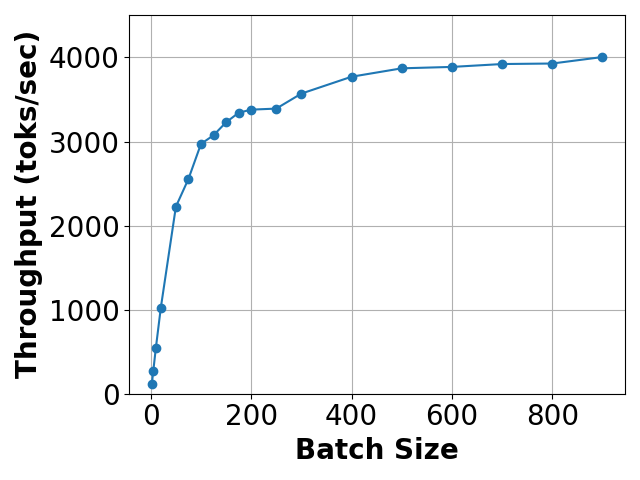
\includegraphics[width=\columnwidth]{results/throughput_vs_batch_size_llama8b_small_requests.png}
\caption{Throughput vs Batch Size}
\label{fig:batch_size_tp}
\end{minipage}
\hfill
\begin{minipage}{1\columnwidth}
\centering
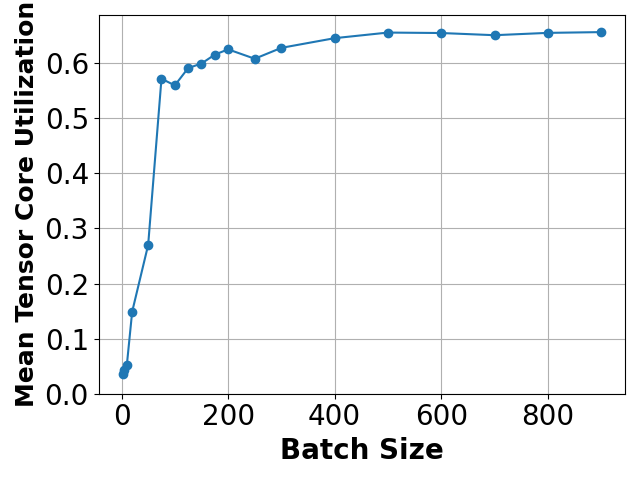
\includegraphics[width=\columnwidth]{results/mean_tenso_vs_batch_size_llama8b_small_requests.png}
\caption{Tensor Core Utilization vs Batch Size}
\label{fig:batch_size_tenso}
\end{minipage}
\hfill
\begin{minipage}{1\columnwidth}
\centering
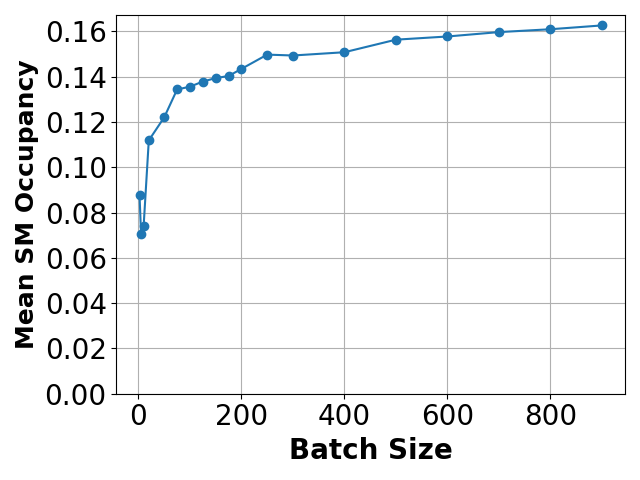
\includegraphics[width=\columnwidth]{results/mean_smocc_vs_batch_size_llama8b_small_requests.png}
\caption{Mean SM Occupancy vs Batch Size}
\label{fig:batch_size_tenso}
\end{minipage}
\end{figure}
\section{Impact of Sharing Position on Decode Throughput - $5L$}


\textcolor{orange}{To further strengthen our observations, we also present results for a sequence length of $5L$ in Figure~\ref{fig:tp_vs_l_1_9_11_5L}, where we extend the length of the top shared nodes by $L$ for all of these settings (the no sharing patterns remain unchanged, with both prefix groups of length $5L$ each).} \textcolor{red}{plot in appendix, but do we need this here?}
\begin{figure}[H]
\centering
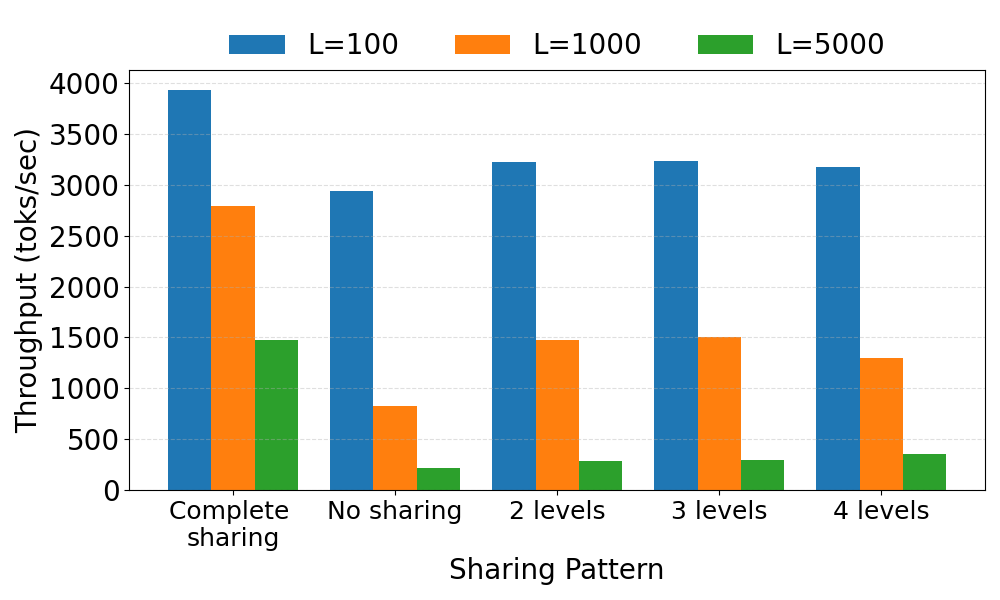
\includegraphics[width=\columnwidth]{results/tp_different_modes_sharing_at_top_5L.png}
\caption{Throughput vs sharing patterns}
\label{fig:tp_vs_l_1_9_11_5L}
\end{figure}


\section{Homo vs Hetero - No Warmup - Varying Decode Tokens}
\label{sec:homo_hetero_no_warmup}

\begin{figure}[H]
\centering
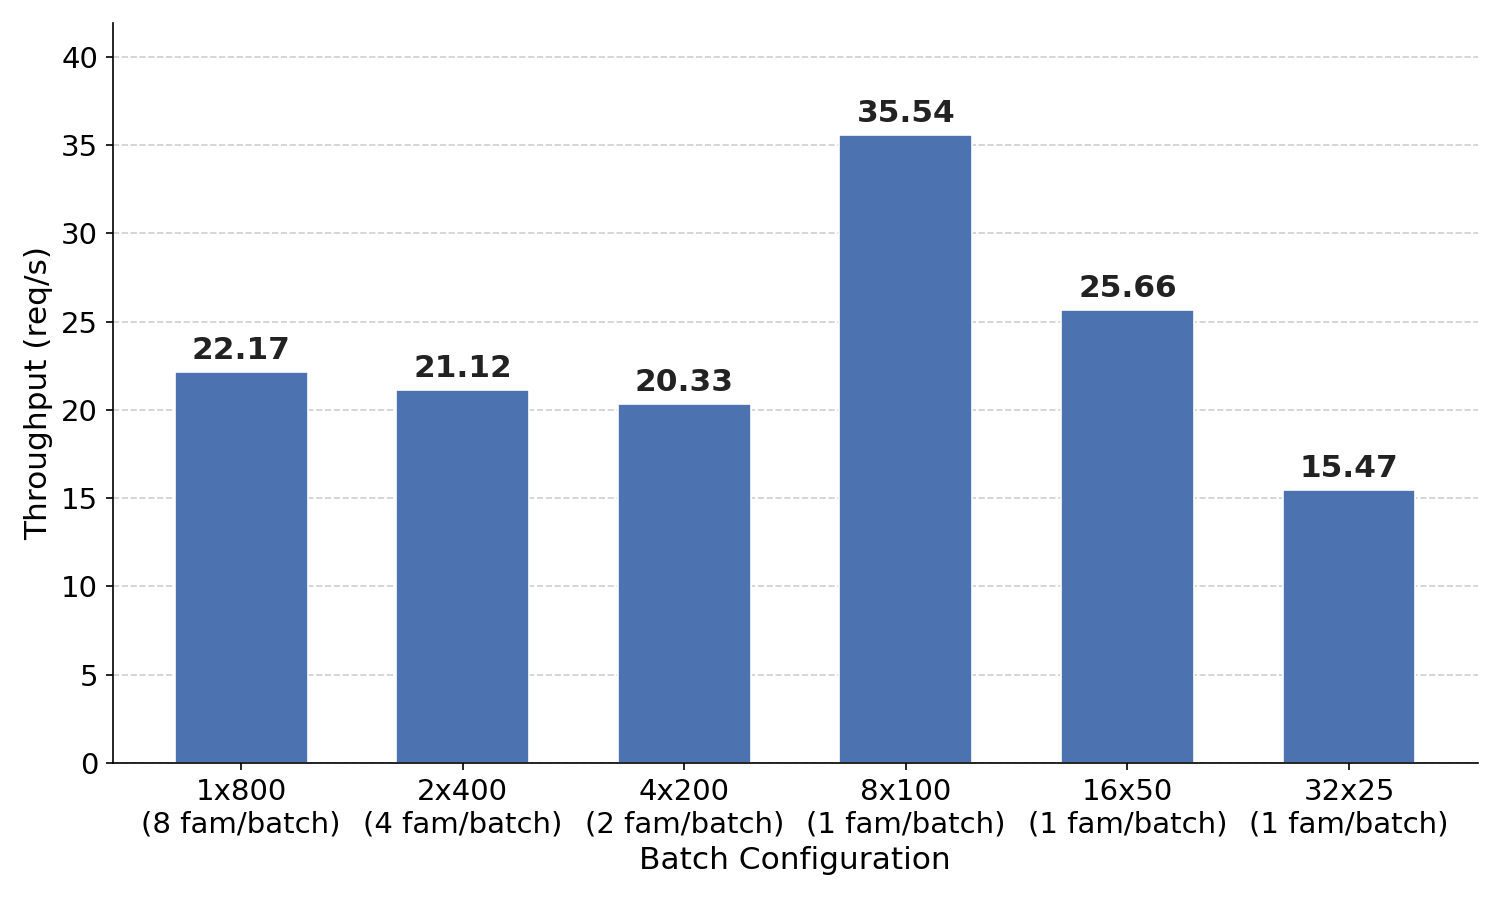
\includegraphics[width=0.8\columnwidth]{results/homo_hetero_throughput_barchart.png}
\caption{with warmup - 50 decode tokens}
\label{fig:homo_hetero_tp_001}
\end{figure}


\begin{figure}[H]
\centering
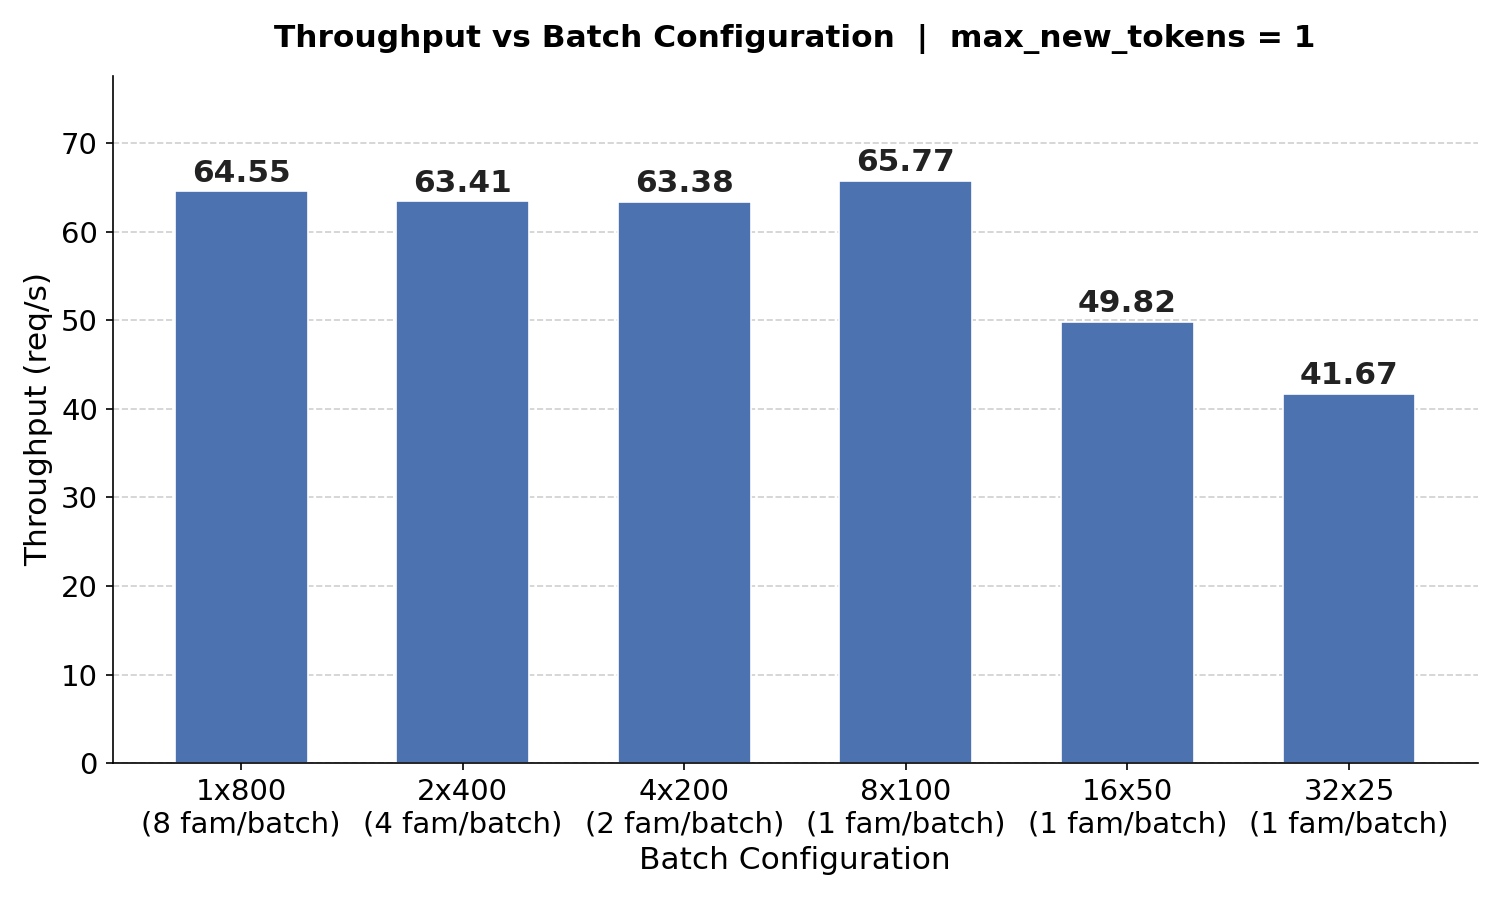
\includegraphics[width=0.8\columnwidth]{results/homo_hetero_throughput_barchart_no_warmup_tok001.png}
\caption{Throughput vs Batch Configuration}
\label{fig:homo_hetero_tp_001}
\end{figure}


\begin{figure}[H]
\centering
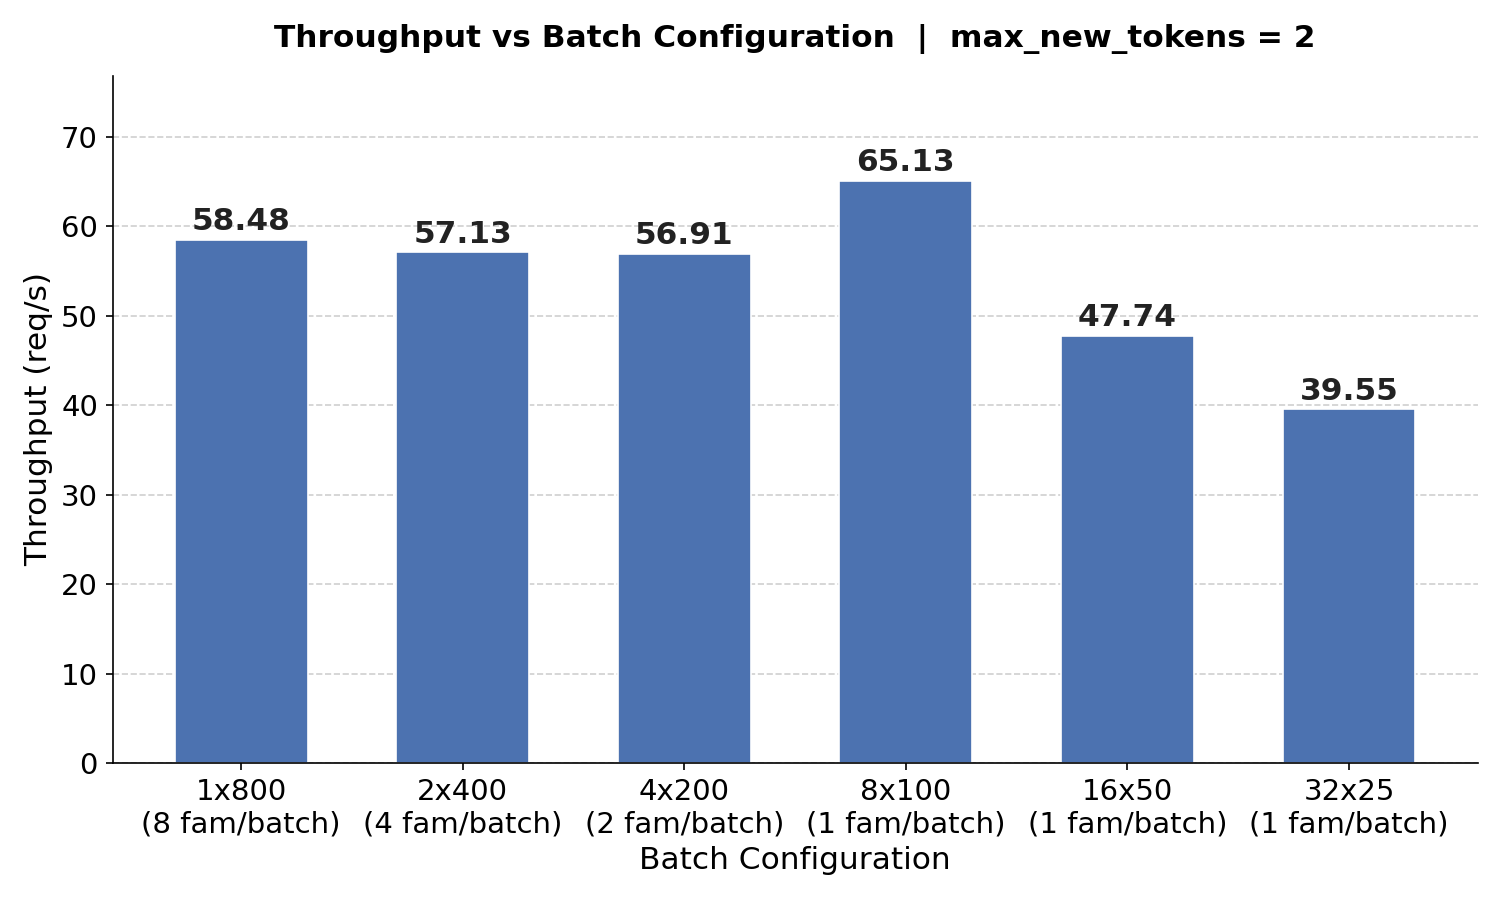
\includegraphics[width=0.8\columnwidth]{results/homo_hetero_throughput_barchart_no_warmup_tok002.png}
\caption{Throughput vs Batch Configuration}
\label{fig:homo_hetero_tp_002}
\end{figure}

\begin{figure}[H]
\centering
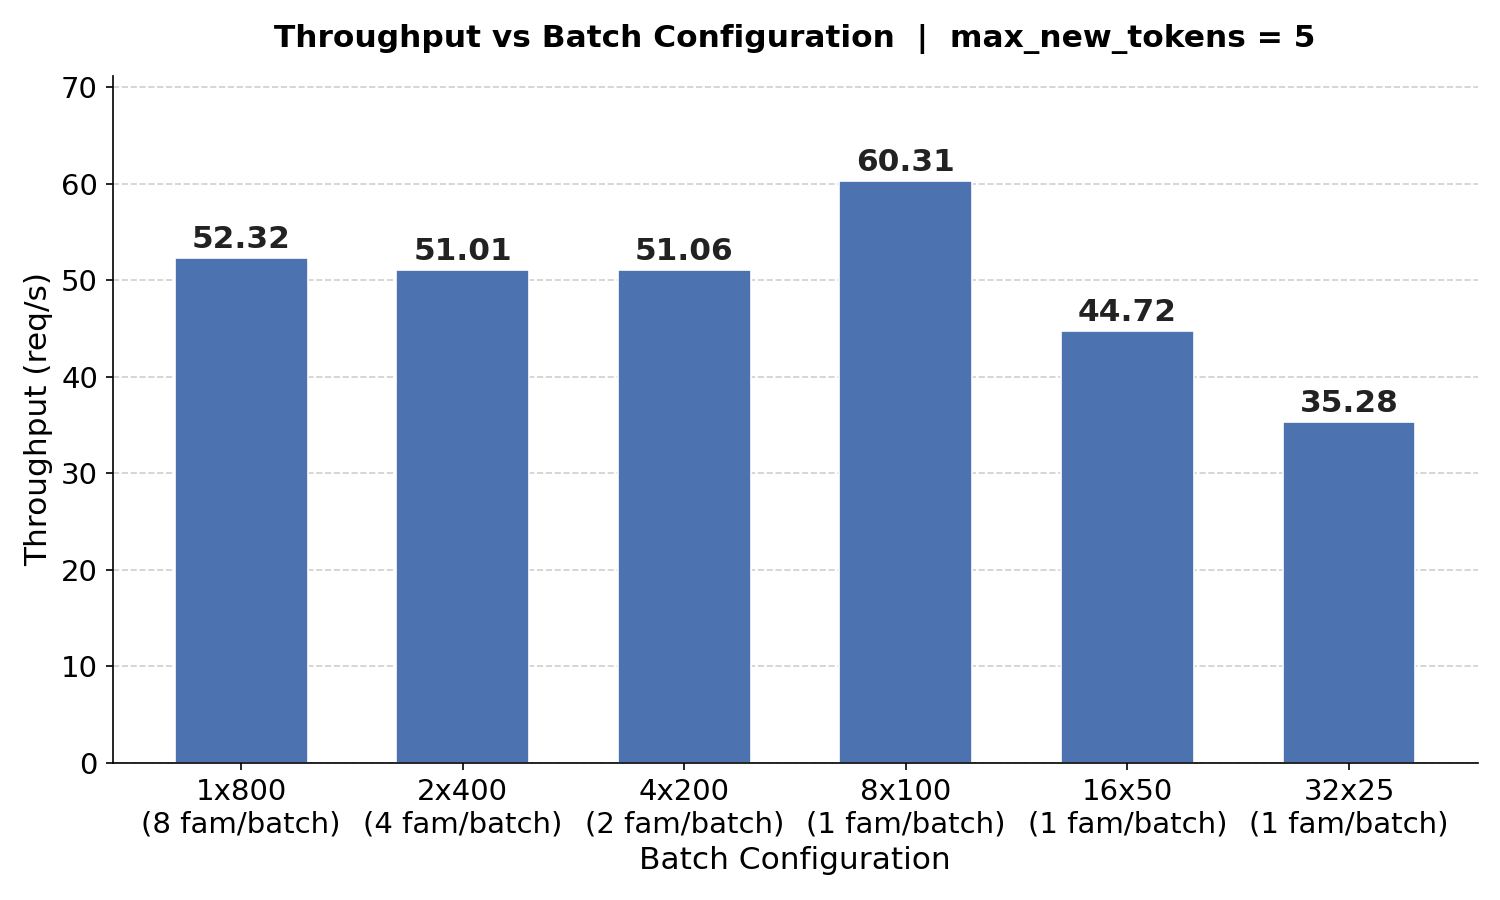
\includegraphics[width=0.8\columnwidth]{results/homo_hetero_throughput_barchart_no_warmup_tok005.png}
\caption{Throughput vs Batch Configuration}
\label{fig:homo_hetero_tp_005}
\end{figure}

\begin{figure}[H]
\centering
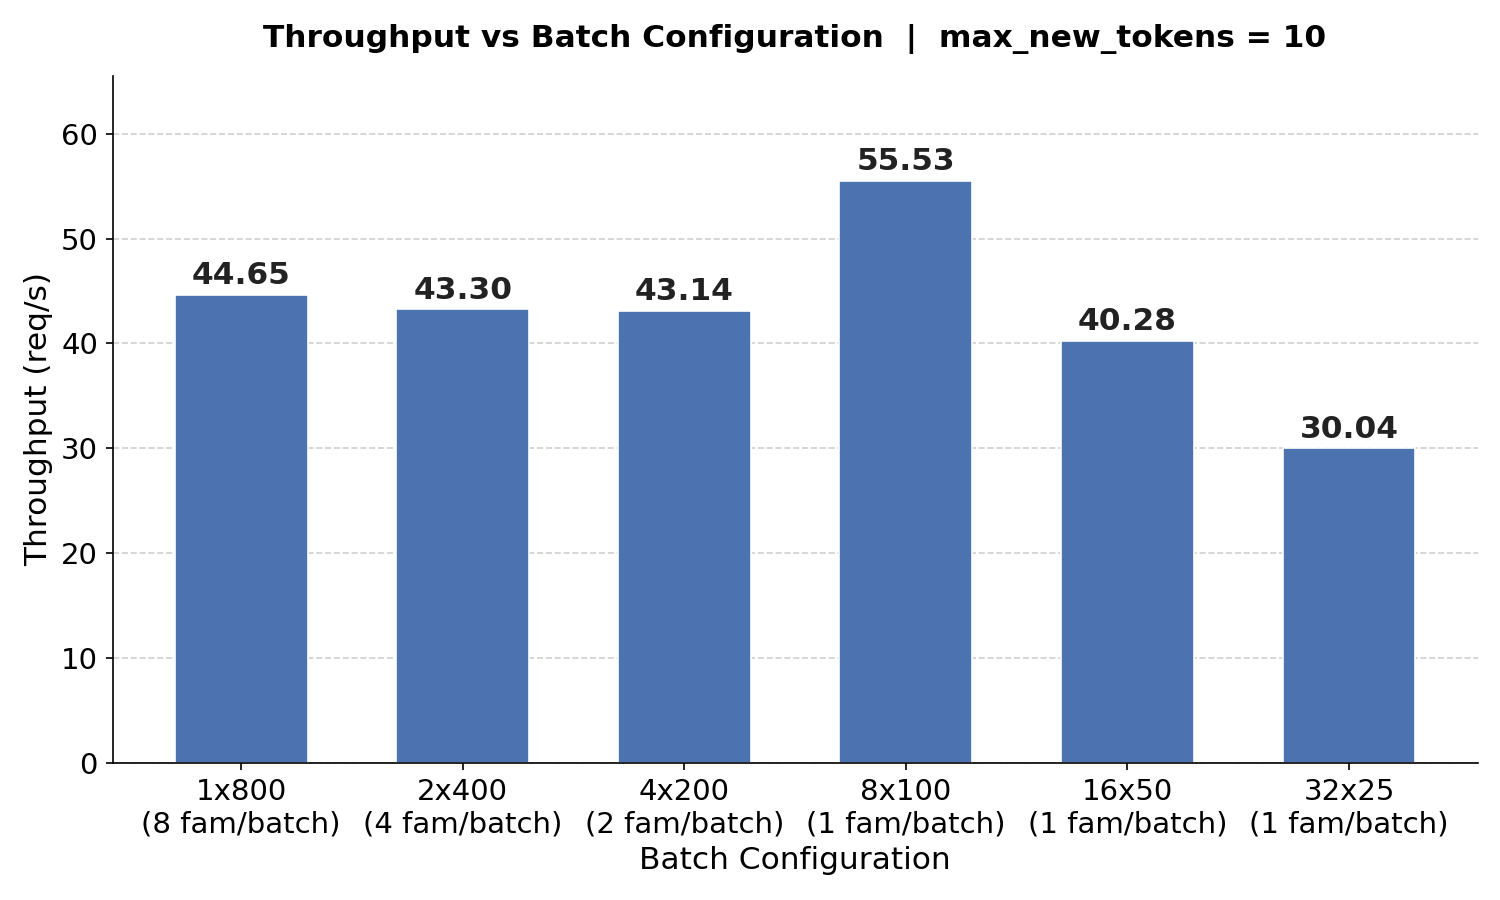
\includegraphics[width=0.8\columnwidth]{results/homo_hetero_throughput_barchart_no_warmup_tok010.png}
\caption{Throughput vs Batch Configuration}
\label{fig:homo_hetero_tp_010}
\end{figure}

\begin{figure}[H]
\centering
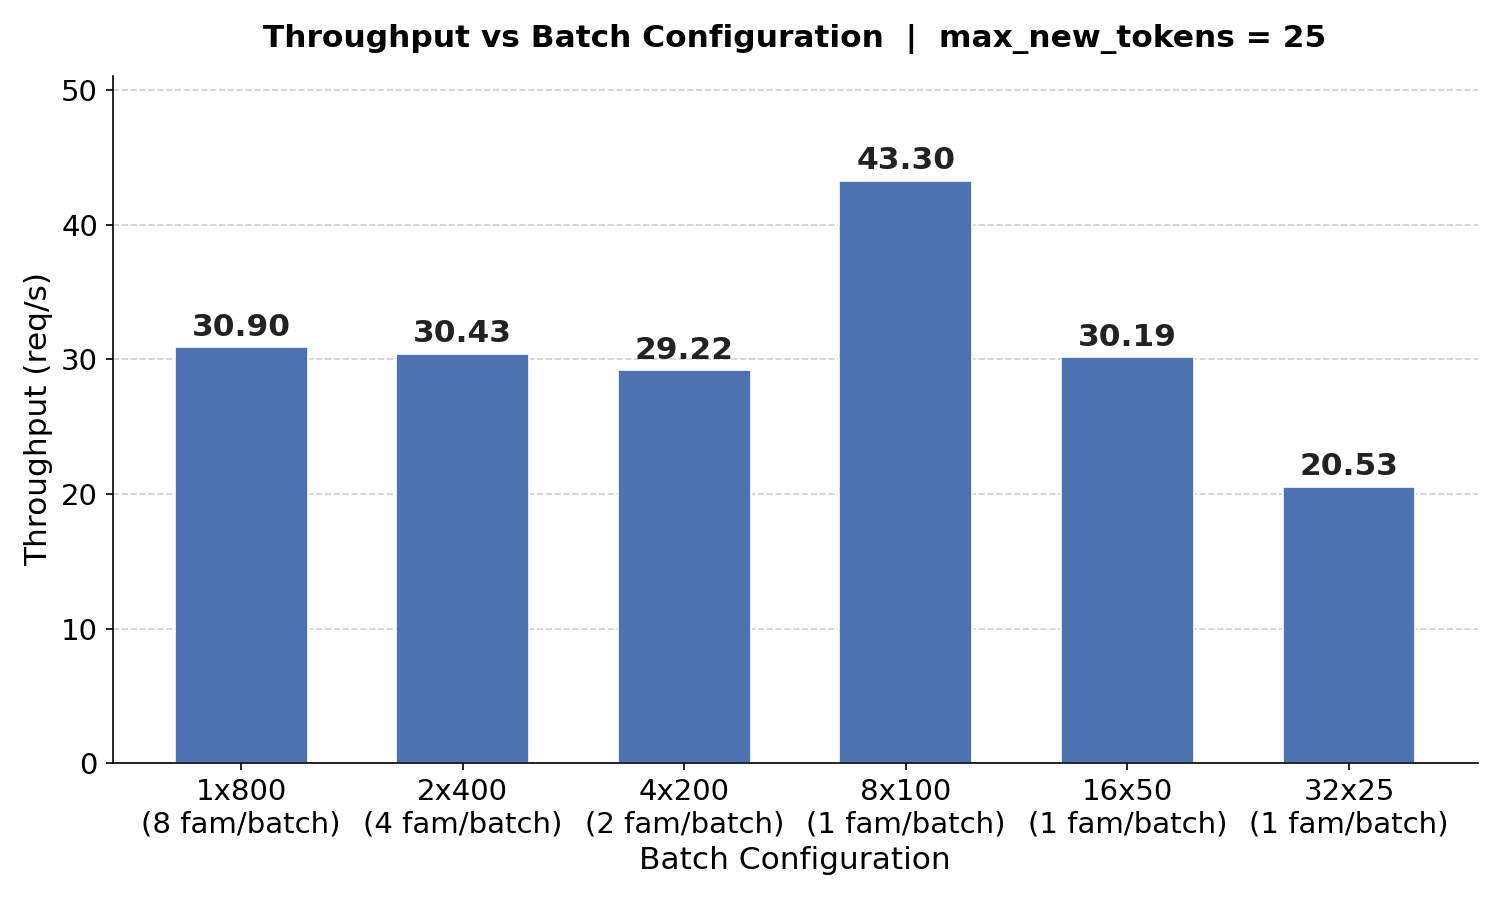
\includegraphics[width=0.8\columnwidth]{results/homo_hetero_throughput_barchart_no_warmup_tok025.png}
\caption{Throughput vs Batch Configuration}
\label{fig:homo_hetero_tp_025}
\end{figure}

\begin{figure}[H]
\centering
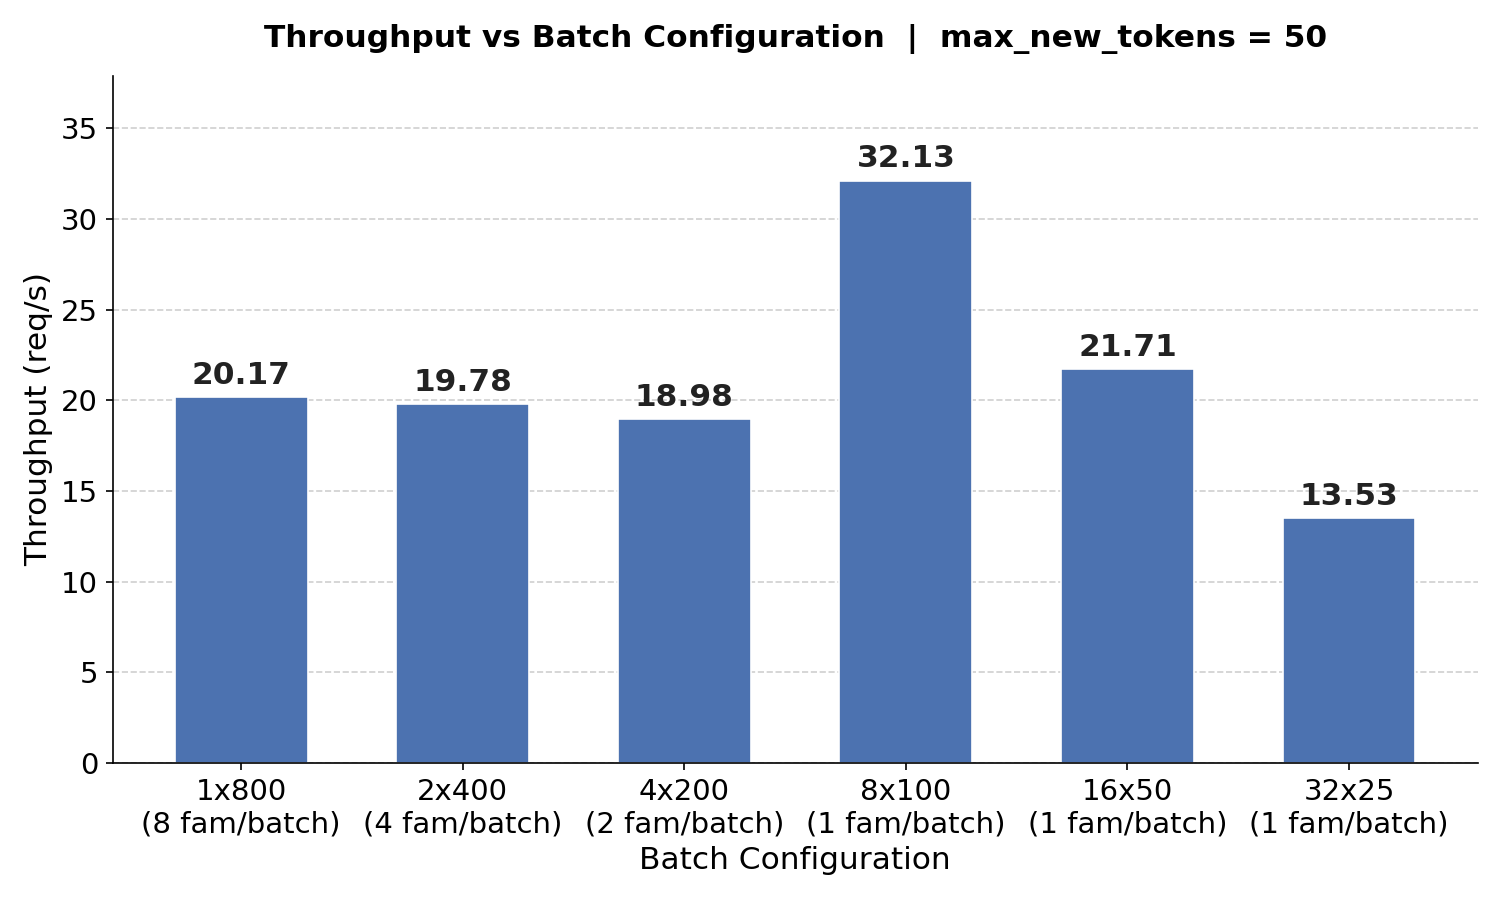
\includegraphics[width=0.8\columnwidth]{results/homo_hetero_throughput_barchart_no_warmup_tok050.png}
\caption{Throughput vs Batch Configuration}
\label{fig:homo_hetero_tp_050}
\end{figure}

\begin{figure}[H]
\centering
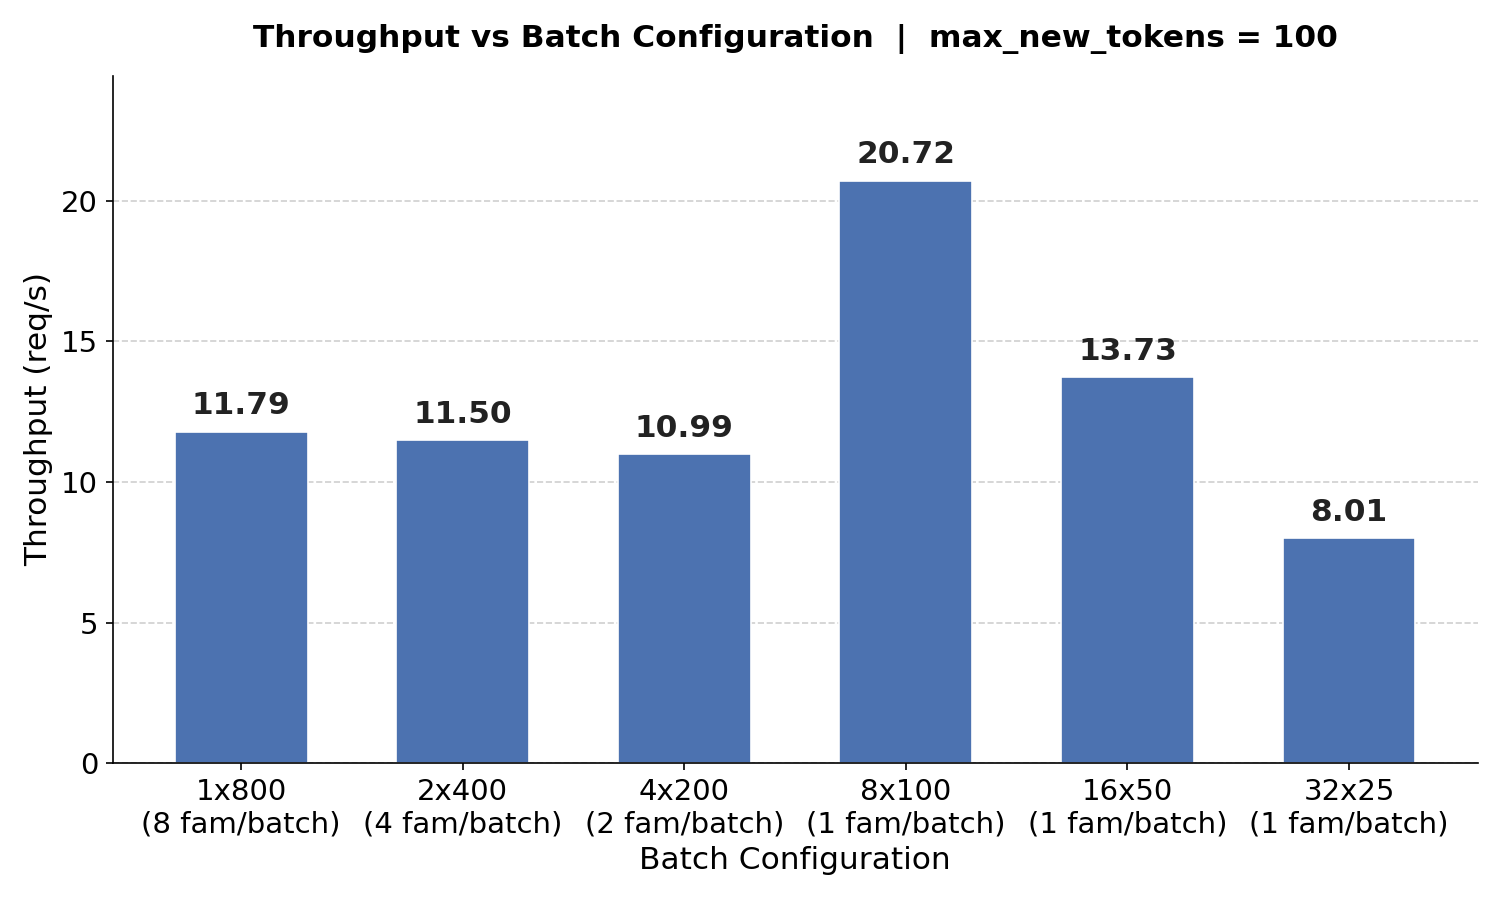
\includegraphics[width=0.8\columnwidth]{results/homo_hetero_throughput_barchart_no_warmup_tok100.png}
\caption{Throughput vs Batch Configuration}
\label{fig:homo_hetero_tp_100}
\end{figure}

\begin{figure}[H]
\centering
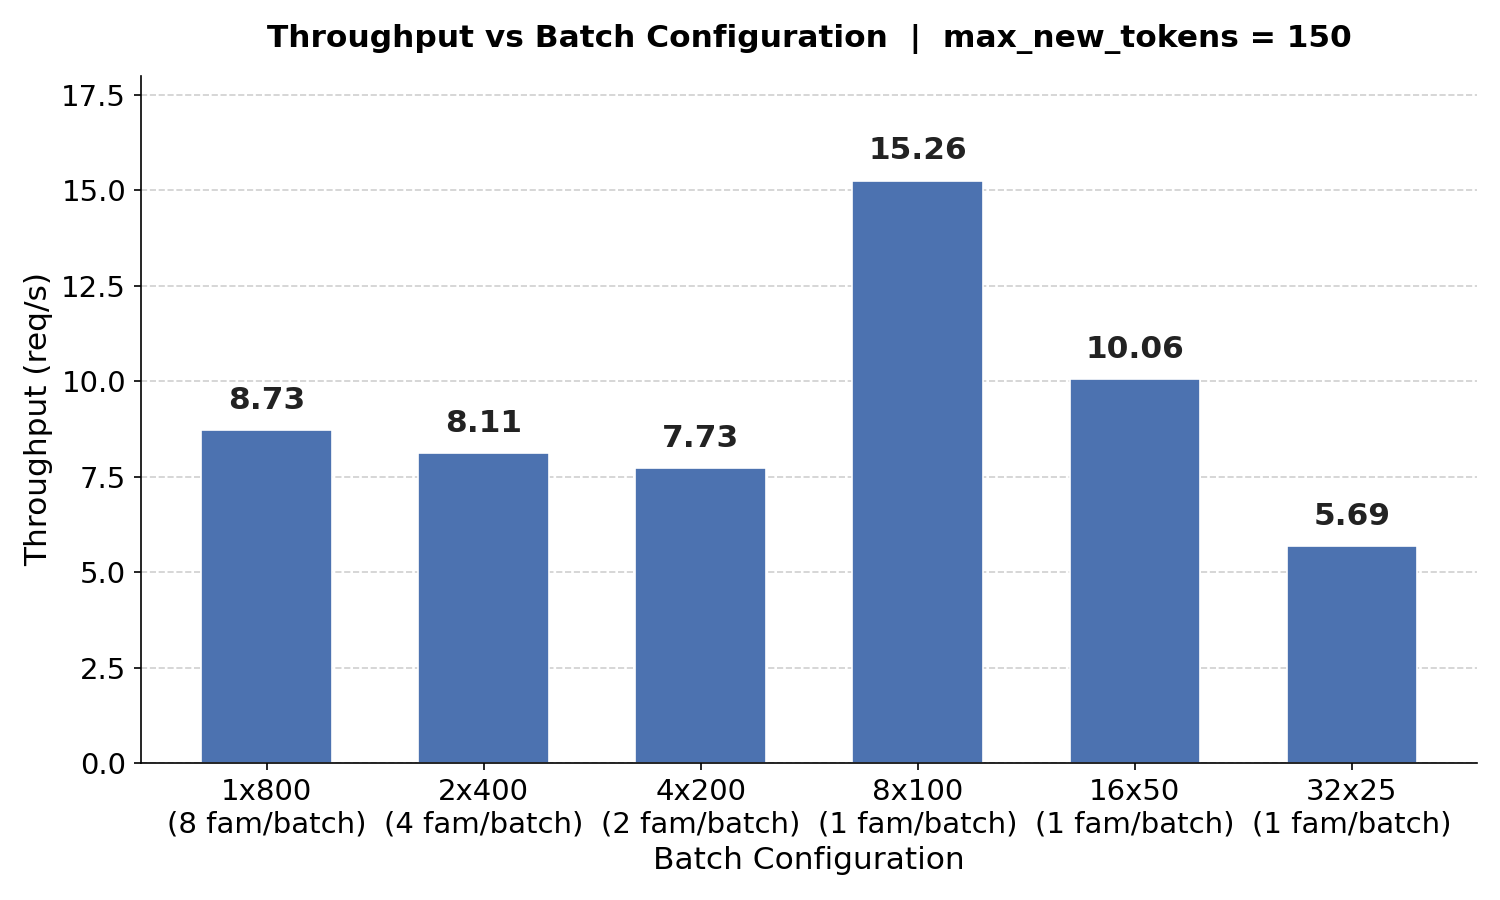
\includegraphics[width=0.8\columnwidth]{results/homo_hetero_throughput_barchart_no_warmup_tok150.png}
\caption{Throughput vs Batch Configuration}
\label{fig:homo_hetero_tp_150}
\end{figure}

\begin{figure}[H]
\centering
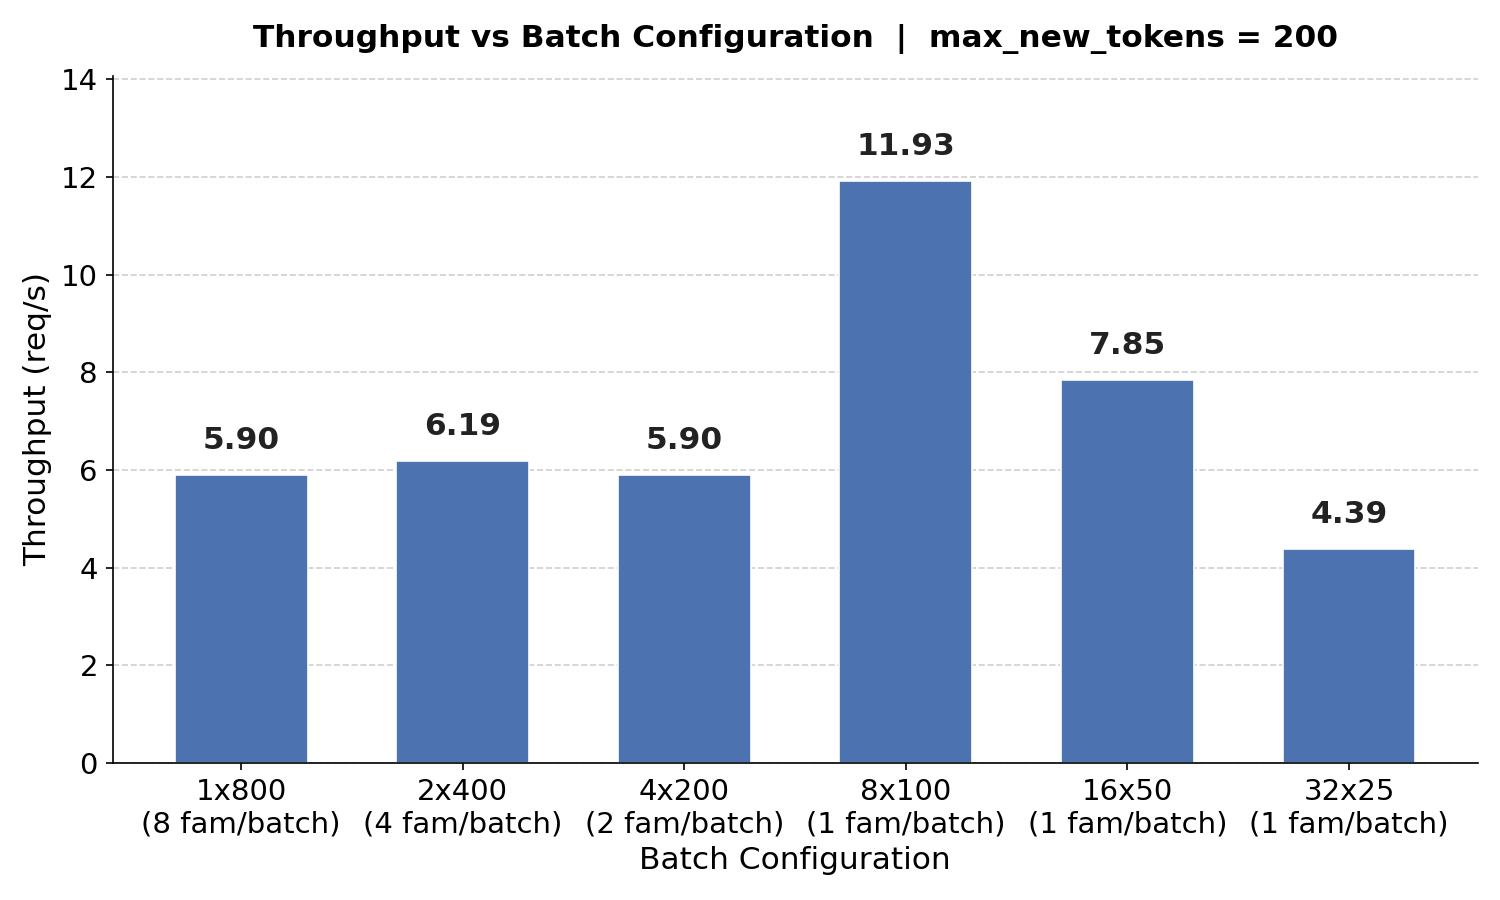
\includegraphics[width=0.8\columnwidth]{results/homo_hetero_throughput_barchart_no_warmup_tok200.png}
\caption{Throughput vs Batch Configuration}
\label{fig:homo_hetero_tp_200}
\end{figure}

\begin{figure}[H]
\centering
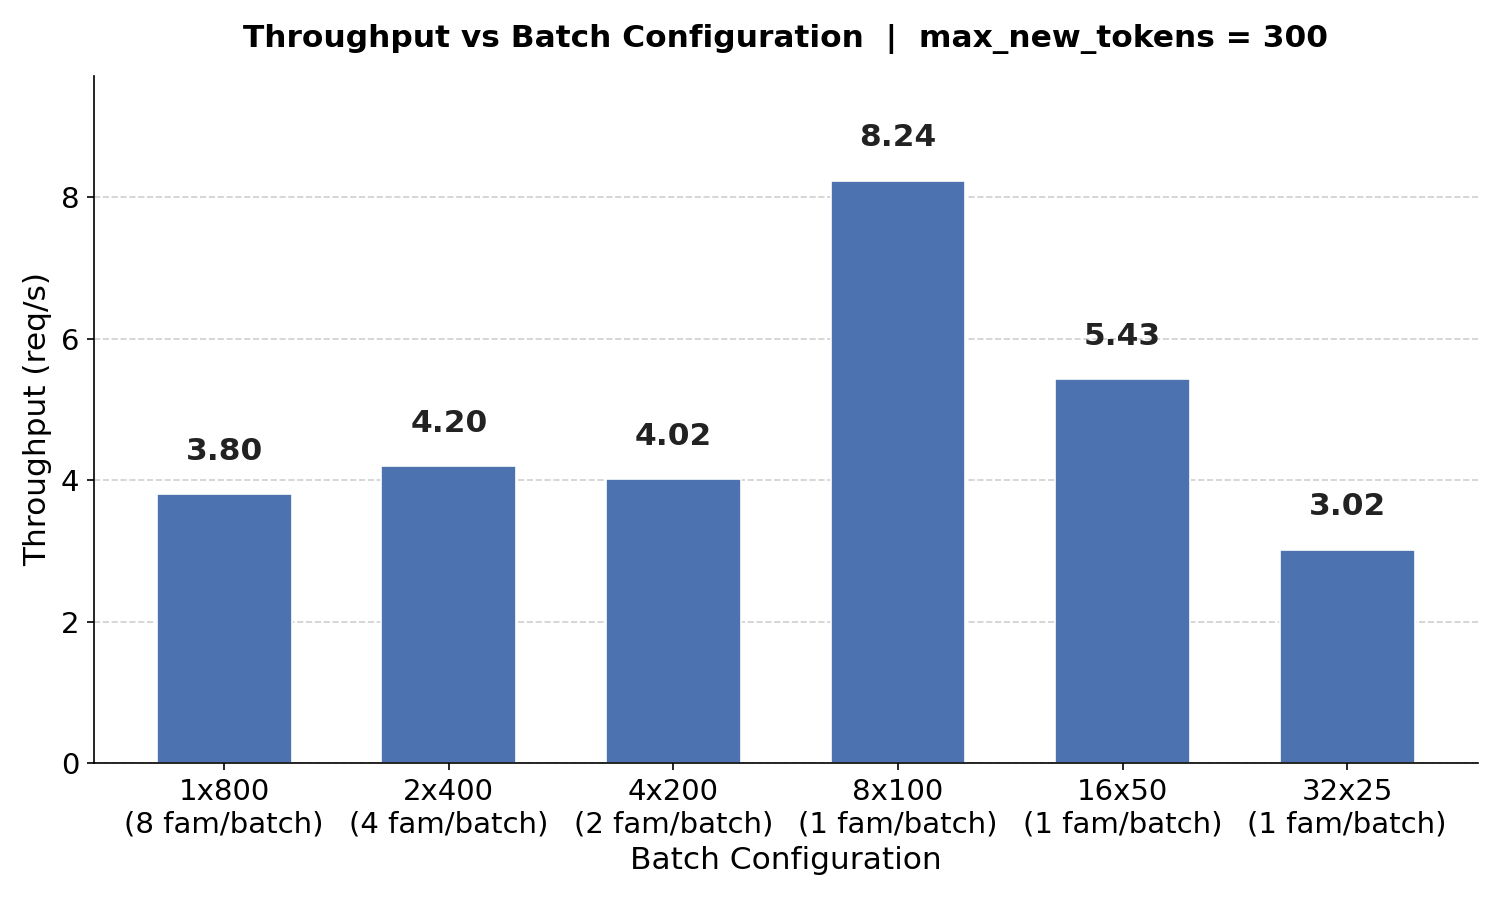
\includegraphics[width=0.8\columnwidth]{results/homo_hetero_throughput_barchart_no_warmup_tok300.png}
\caption{Throughput vs Batch Configuration}
\label{fig:homo_hetero_tp_300}
\end{figure}


\section{Mean SM Occupancy vs Batch Size}
\begin{figure}[H]
\centering
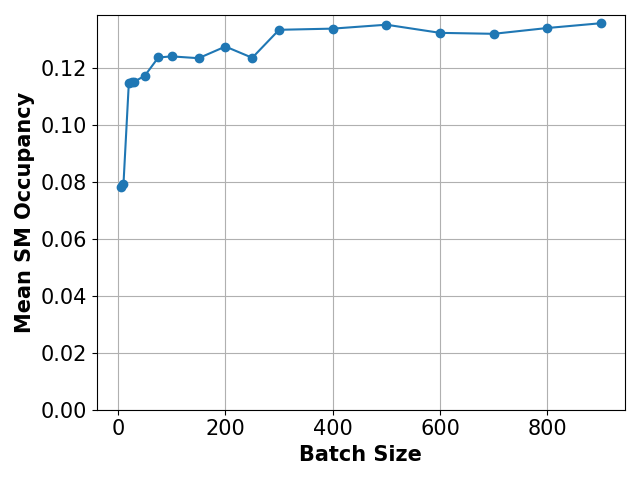
\includegraphics[width=\columnwidth]{results/mean_smocc_vs_batch_size_llama8b.png}
\caption{SM Occupancy}
\label{fig:batch_size_smocc}
\end{figure}

\section{Cache Working Set Size Theory}
\begin{figure}[H]
\centering
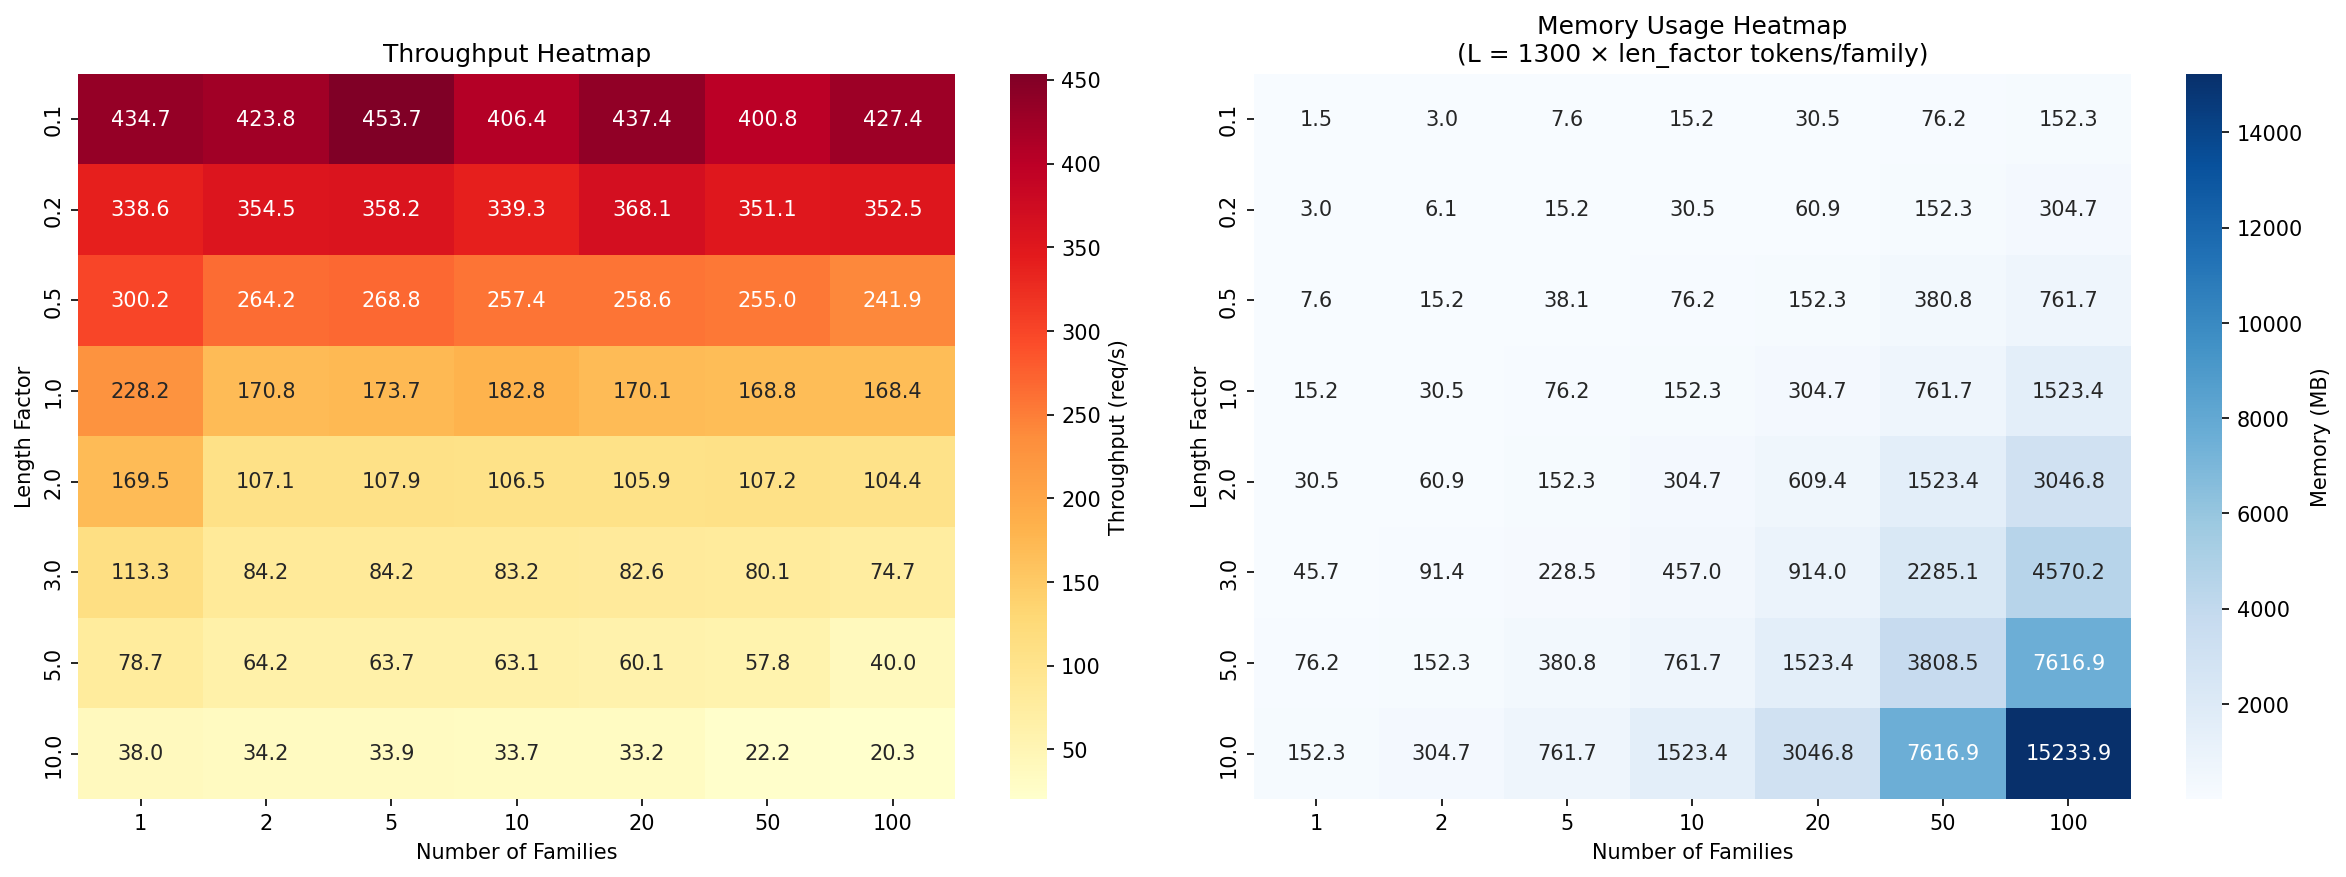
\includegraphics[width=\columnwidth]{results/qwen_families_lengths_tp_mem.png}
\caption{QWEN Throughput and KV Cache Memory across various sequence lengths and number of families}
\label{fig:qwen_fam_len_tp_mem}
\end{figure}



\newpage
\textcolor{red}{\LARGE DUMP APPENDIX STARTS HERE!!!}
\section{Radix Tree Workload Modes}

    \begin{tikzpicture}[
    box/.style={rectangle, draw, minimum width=1cm, minimum height=0.6cm, anchor=west},
    label/.style={font=\small}
]
    \node[font=\Large\bfseries] at (0,2) {Full Sharing (All share 3L)};
    
    \node[label] at (0,0.5) {All requests:};
    
    \node[box, fill=shared1, minimum width=6cm] (s1) at (1,0.5) {};
    \node[label, white, font=\bfseries] at (s1.center) {Shared 3L};
    
    \draw[decorate, decoration={brace, amplitude=5pt, mirror}] 
        (1,-0.2) -- (7,-0.2) node[midway, below=5pt, font=\footnotesize] {3L tokens};
\end{tikzpicture}

    \hspace*{+1cm}
    \begin{tikzpicture}[
    box/.style={rectangle, draw, minimum width=1cm, minimum height=0.6cm, anchor=west},
    label/.style={font=\small}
]
    \node[font=\Large\bfseries] at (2,3.5) {All share 2L, then 2xL};
    
    % Level 1: All share
    \node[label] at (0,2) {All requests:};
    \node[box, fill=shared1, minimum width=4cm] (l1) at (1,2) {};
    \node[label, white, font=\bfseries] at (l1.center) {Shared 2L};
    
    % Level 2: Two groups
    \node[label] at (0,0.8) {Group 1:};
    \node[box, fill=shared1, minimum width=4cm] at (1,0.8) {};
    \node[box, fill=unique1, minimum width=2cm] at (5,0.8) {};
    \node[label, white] at (3,0.8) {Shared 2L};
    \node[label, white] at (6,0.8) {+L unique};
    
    \node[label] at (0,0) {Group 2:};
    \node[box, fill=shared1, minimum width=4cm] at (1,0) {};
    \node[box, fill=unique2, minimum width=2cm] at (5,0) {};
    \node[label, white] at (3,0) {Shared 2L};
    \node[label, white] at (6,0) {+L unique};
    
    % Annotations
    \draw[decorate, decoration={brace, amplitude=5pt, mirror}] 
        (1,-0.7) -- (5,-0.7) node[midway, below=5pt, font=\footnotesize] {2L};
    \draw[decorate, decoration={brace, amplitude=5pt, mirror}] 
        (5,-0.7) -- (7,-0.7) node[midway, below=5pt, font=\footnotesize] {L};
    
    % Arrow showing split
    \draw[->, thick] (5,1.7) -- (5,1.1);
    \node[font=\footnotesize] at (6.5,1.4) {Split into 2 groups};
    
\end{tikzpicture}


    \hspace*{0cm}
    \begin{tikzpicture}[
    box/.style={rectangle, draw, minimum width=1cm, minimum height=0.6cm, anchor=west},
    label/.style={font=\small}
]
    \node[font=\Large\bfseries] at (1.5,3.5) {All share L, then 2x2L};
    
    \node[label] at (0,2) {All requests:};
    \node[box, fill=shared1, minimum width=2cm] (l1) at (3,2) {};
    \node[label, white, font=\bfseries] at (l1.center) {Shared L};
    
    \node[label] at (0,0.8) {Group 1:};
    \node[box, fill=shared1, minimum width=2cm] at (3,0.8) {};
    \node[box, fill=unique1, minimum width=4cm] at (5,0.8) {};
    \node[label, white] at (4,0.8) {L};
    \node[label, white] at (7,0.8) {+2L unique};
    
    \node[label] at (0,0) {Group 2:};
    \node[box, fill=shared1, minimum width=2cm] at (3,0) {};
    \node[box, fill=unique2, minimum width=4cm] at (5,0) {};
    \node[label, white] at (4,0) {L};
    \node[label, white] at (7,0) {+2L unique};
    
    \draw[decorate, decoration={brace, amplitude=5pt, mirror}] 
        (3,-0.7) -- (5,-0.7) node[midway, below=5pt, font=\footnotesize] {L};
    \draw[decorate, decoration={brace, amplitude=5pt, mirror}] 
        (5,-0.7) -- (9,-0.7) node[midway, below=5pt, font=\footnotesize] {2L};
    
    \draw[->, thick] (4,1.7) -- (4,1.1);
    \node[font=\footnotesize] at (5.5,1.4) {Split into 2 groups};
    
\end{tikzpicture}



    \begin{tikzpicture}[
    box/.style={rectangle, draw, minimum width=0.8cm, minimum height=0.5cm, anchor=west},
    label/.style={font=\small},
    level distance=1.2cm,
    level 1/.style={sibling distance=6cm},
    level 2/.style={sibling distance=3cm}
]
    \node[font=\Large\bfseries] at (3,5) {Three-Level Tree (L → 2L → 3L, 4 leaves)};
    
    \node[label] at (0,3.5) {Level 1:};
    \node[box, fill=shared1, minimum width=2cm] at (2,3.5) {};
    \node[label, white] at (3,3.5) {L (all share)};
    
    \node[label] at (0,2) {Level 2:};
    \node[box, fill=shared1, minimum width=2cm] at (2,2) {};
    \node[box, fill=shared2, minimum width=2cm] at (4.5,2) {};
    \node[label, white, font=\footnotesize] at (3,2) {Branch 1};
    \node[label, white, font=\footnotesize] at (5.5,2) {Branch 2};
    \node[font=\footnotesize] at (3,1.6) {+L};
    \node[font=\footnotesize] at (5.5,1.6) {+L};
    
    \node[label] at (0,0.5) {Level 3:};
    \node[box, fill=unique1, minimum width=1.2cm] at (1.5,0.5) {};
    \node[box, fill=unique2, minimum width=1.2cm] at (3,0.5) {};
    \node[box, fill=unique3, minimum width=1.2cm] at (5,0.5) {};
    \node[box, fill=unique4, minimum width=1.2cm] at (6.5,0.5) {};
    
    \node[label, white, font=\tiny] at (2.1,0.5) {Leaf 1};
    \node[label, white, font=\tiny] at (3.6,0.5) {Leaf 2};
    \node[label, white, font=\tiny] at (5.6,0.5) {Leaf 3};
    \node[label, white, font=\tiny] at (7.1,0.5) {Leaf 4};
    
    \node[font=\tiny] at (2.1,0.1) {+L};
    \node[font=\tiny] at (3.6,0.1) {+L};
    \node[font=\tiny] at (5.6,0.1) {+L};
    \node[font=\tiny] at (7.1,0.1) {+L};
    
    \draw[->, thick] (3,3.2) -- (3,2.3);
    \draw[->, thick] (3,3.2) -- (5.5,2.3);
    \draw[->, thick] (3,1.7) -- (2.1,0.8);
    \draw[->, thick] (3,1.7) -- (3.6,0.8);
    \draw[->, thick] (5.5,1.7) -- (5.6,0.8);
    \draw[->, thick] (5.5,1.7) -- (7.1,0.8);
\end{tikzpicture}


    \begin{tikzpicture}[
    box/.style={rectangle, draw, minimum width=1cm, minimum height=0.6cm, anchor=west},
    label/.style={font=\small}
]
    \node[font=\Large\bfseries] at (3,3) {2 separate groups with 3L each};
    
    \node[label] at (0,1.5) {Group 1:};
    \node[box, fill=unique1, minimum width=6cm] at (3,1.5) {};
    \node[label, white, font=\bfseries] at (6,1.5) {Context A (3L tokens)};
    
    \node[label] at (0,0.5) {Group 2:};
    \node[box, fill=unique2, minimum width=6cm] at (3,0.5) {};
    \node[label, white, font=\bfseries] at (6,0.5) {Context B (3L tokens)};

    \draw[decorate, decoration={brace, amplitude=5pt, mirror}] 
        (3,-0.2) -- (9,-0.2) node[midway, below=5pt, font=\footnotesize] {3L tokens (completely different)};
\end{tikzpicture}


    \begin{figure}
        \centering
    \includegraphics[width=\columnwidth]{\RESULTDIR/radix_tree_workloads_results.png}
    \captionof{figure}{Results across varying L}
\end{figure}


{Mode 6}
    \begin{tikzpicture}[
    box/.style={rectangle, draw, minimum width=0.4cm, minimum height=0.5cm, anchor=west},
    label/.style={font=\small}
]
    \node[font=\Large\bfseries] at (5,4) {2.5L shared + 10x0.5L};
    
    \node[label] at (2,2.5) {All requests:};
    \node[box, fill=shared1, minimum width=4cm] at (3,2.5) {};
    \node[label, white, font=\bfseries] at (4.8,2.5) {Shared 2.5L};
    
    \node[label] at (2,1) {10 groups};
    
    \foreach \x/\col in {0/unique1, 1/unique2, 2/unique3, 3/unique4, 4/unique1, 5/unique2, 6/unique3, 7/unique4, 8/unique1, 9/unique2} {
        \node[box, fill=shared1, minimum width=4cm] at (3+\x*0.5,1-\x*0.15) {};
        \node[box, fill=\col, minimum width=1cm] at (7+\x*0.5,1-\x*0.15) {};
    }
    
    \draw[decorate, decoration={brace, amplitude=5pt, mirror}] 
        (3,-1.0) -- (8,-1.0) node[midway, below=5pt, font=\footnotesize] {2.5L};
    \draw[decorate, decoration={brace, amplitude=5pt, mirror}] 
        (8,-1.0) -- (9,-1.0) node[midway, below=5pt, font=\footnotesize] {0.5L};
    
    \draw[->, thick] (5.5,2.2) -- (5.5,1.4);
    \node[font=\footnotesize] at (7,1.8) {Split into 10 groups};
\end{tikzpicture}


{Mode 7}
    \begin{tikzpicture}[
    box/.style={rectangle, draw, minimum width=0.3cm, minimum height=0.4cm, anchor=west},
    label/.style={font=\small}
]
    \node[font=\Large\bfseries\sffamily] at (4,4) {2.8L shared + 50x0.2L};

    
    \node[label] at (2,2.5) {All requests:};
    \node[box, fill=shared1, minimum width=4cm] at (3,2.5) {};
    \node[label, white, font=\bfseries] at (5,2.5) {Shared 2.8L};
    \node[label] at (2,1) {50 groups};
    
    \foreach \x/\col in {0/unique1, 1/unique2, 2/unique3, 3/unique4, 4/unique1, 5/unique2, 6/unique3, 7/unique4, 8/unique1, 9/unique2, 10/unique3, 11/unique4, 12/unique1, 13/unique2, 14/unique3} {
        \node[box, fill=shared1, minimum width=4cm] at (3+\x*0.3,1-\x*0.08) {};
        \node[box, fill=\col, minimum width=0.4cm] at (7+\x*0.3,1-\x*0.08) {};
    }
    
    \node[font=\footnotesize] at (7,-0.5) {...(More groups)};
    
    \draw[decorate, decoration={brace, amplitude=5pt, mirror}] 
        (3,-1.2) -- (9.6,-1.2) node[midway, below=5pt, font=\footnotesize] {2.8L};
    \draw[decorate, decoration={brace, amplitude=5pt, mirror}] 
        (9.6,-1.2) -- (10,-1.2) node[midway, below=5pt, font=\footnotesize] {0.2L};
    
\end{tikzpicture}



{Mode 8}
    \begin{tikzpicture}[
    box/.style={rectangle, draw, minimum width=0.3cm, minimum height=0.4cm, anchor=west},
    label/.style={font=\small}
]
    \node[font=\Large\bfseries] at (5,4) {0.2L shared + 50x2.8L};
    
    \node[label] at (1.5,2.5) {All requests:};
    \node[box, fill=shared1, minimum width=0.4cm] at (3,2.5) {};
    \node[label, font=\footnotesize] at (3.2,2.5) {0.2L};
    
    \node[label] at (1.5,1) {50 groups};
    
    \foreach \x/\col in {0/unique1, 1/unique2, 2/unique3, 3/unique4, 4/unique1, 5/unique2, 6/unique3, 7/unique4, 8/unique1, 9/unique2, 10/unique3, 11/unique4, 12/unique1, 13/unique2, 14/unique3} {
        \node[box, fill=shared1, minimum width=0.4cm] at (3+\x*0.35,1-\x*0.08) {};
        \node[box, fill=\col, minimum width=4cm] at (3.4+\x*0.35,1-\x*0.08) {};
    }
    
    \node[font=\footnotesize] at (6.5,-0.5) {...(More groups)};
    
    \draw[decorate, decoration={brace, amplitude=5pt, mirror}] 
        (3,-1.2) -- (3.4,-1.2) node[midway, below=5pt, font=\footnotesize] {0.2L};
    \draw[decorate, decoration={brace, amplitude=5pt, mirror}] 
        (3.4,-1.2) -- (9,-1.2) node[midway, below=5pt, font=\footnotesize] {2.8L};
\end{tikzpicture}



{Comparison of Throughput across different modes}
\begin{table}[h!]
\centering
\begin{tabular}{|l|c|c|}
\hline
\textbf{Modes} & \textbf{L = 1000} & \textbf{L = 2000} \\
\hline
Mode 1 - All share 3L & 29.18 & 27.97 \\
Mode 2 - All share 2L, then 2xL & 19.94 & 14.06 \\
Mode 3 - All share L, then 2x2L& 15.40 & 8.89 \\
Mode 4 - L $\rightarrow$ 2L $\rightarrow$ 3L, 4 leaves& 15.41 & 9.88 \\
Mode 5 - 2 separate groups with 3L each & 10.18 & 6.62 \\
Mode 6 - 2.5L shared + 10x0.5L & 25.34 & 20.27 \\
Mode 7 - 2.8L shared + 50x0.2L & 28.05 & 23.17 \\
Mode 8 - 0.2L shared + 50x2.8L & 10.05 & 6.48 \\
\hline
\end{tabular}
\caption{Comparison of Throughput across different modes}
\end{table}



\section{Finding the Sweet Zone}
{How many families?}
\begin{itemize}
    \item A high request arrival rate (500 req/sec)
    \item Max batch size of 500
    \item A shared prefix of length 6500 tokens
    \item 100 new output tokens 
    \item Model: Llama3.1-8B
\end{itemize}
\begin{table}
\centering
\resizebox{\columnwidth}{!}{
\begin{tabular}{|c|cc|cc|}
\hline
\multirow{2}{*}{Number of Families} 
& \multicolumn{2}{c|}{vLLM Baseline (FCFS)} 
& \multicolumn{2}{c|}{vLLM (User-provided Family IDs)} \\
\cline{2-5}
& Average Batch Size & Throughput 
& Average Batch Size & Throughput \\
\hline
10  & 465.48  & 5.92 & 141.23 & 21.94 \\
20  & 455.47 & 5.74 & 72.67 & 15.27 \\
50  & 57.48 & 2.07 & 64.77 & 14.84 \\
100 & 41.97 & 1.11 & 67.14 & 14.82 \\
\hline
\end{tabular}
}
\end{table}



{How many req/sec?}
\begin{itemize}
    \item 5 families
    \item Max batch size of 500
    \item A shared prefix of length 6500 tokens
    \item 100 new output tokens 
    \item Model: Llama3.1-8B
\end{itemize}
\begin{table}
\centering
\resizebox{\columnwidth}{!}{
\begin{tabular}{|c|cc|cc|}
\hline
\multirow{2}{*}{req/sec} 
& \multicolumn{2}{c|}{vLLM Baseline (FCFS)} 
& \multicolumn{2}{c|}{vLLM (User-provided Family IDs)} \\
\cline{2-5}
& Average Batch Size & Throughput 
& Average Batch Size & Throughput \\
\hline
1  & 2.6  & 1.04 & 2.02 & 0.95 \\
2  & 5.15  & 2.00 & 4.48 & 1.99 \\
\rowcolor{lightgray}
5  & 29.60  & 5.09 & 11.11 & 4.40 \\
10  & 395.80  & 4.42 & 23.96 & 8.16 \\
20  & 438.85  & 5.25 & 52.79 & 13.32 \\
\hline
\end{tabular}
}
\end{table}



{How long should the shared prefix be?}
\begin{itemize}
    \item A high request arrival rate (500 req/sec)
    \item Max batch size of 500
    \item 5 families
    \item 100 new output tokens 
    \item Model: Llama3.1-8B
\end{itemize}
\begin{table}
\centering
\resizebox{\columnwidth}{!}{
\begin{tabular}{|c|cc|cc|}
\hline
\multirow{2}{*}{Shared Prefix Length in Number of Tokens} 
& \multicolumn{2}{c|}{vLLM Baseline (FCFS)} 
& \multicolumn{2}{c|}{vLLM (User-provided Family IDs)} \\
\cline{2-5}
& Average Batch Size & Throughput 
& Average Batch Size & Throughput \\
\hline
13  & 455.48 & 42.47 & 141.23 & 44.67 \\
\rowcolor{lightgray}
65  & 448.87  & 40.14 & 318.60 & 43.96 \\
130  & 460.09  & 38.19 & 330.49 & 41.99 \\
260  & 462.80  & 35.34 & 326.36 & 44.58 \\
650  & 469.12  & 27.47 & 335.21 & 42.00 \\
\hline
\end{tabular}
}
\end{table}


{How large should the model be?}
\begin{itemize}
    \item A high request arrival rate (500 req/sec)
    \item Max batch size of 500
    \item 5 families
    \item 100 new output tokens 
    \item Shared prefix length: 6500 tokens
\end{itemize}
\begin{table}
\centering
\resizebox{\columnwidth}{!}{
\begin{tabular}{|c|cc|cc|}
\hline
\multirow{2}{*}{Model Name} 
& \multicolumn{2}{c|}{vLLM Baseline (FCFS)} 
& \multicolumn{2}{c|}{vLLM (User-provided Family IDs)} \\
\cline{2-5}
& Average Batch Size & Throughput 
& Average Batch Size & Throughput \\
\hline
Qwen2.5-0.5B  & 378.98 & 25.40 & 89.63 & 49.08 \\
Llama3.1-8B  & 448.87  & 4.34 & 151.21 & 30.84 \\
LongChat-13B  & 5.28 & 0.61 & 215.70 & 22.01 \\
\hline
\end{tabular}
}
\end{table}


\section{Other experiments}

{Varying the amount of sharing}
\centering
\begin{tikzpicture}[
    scale=0.85,
    every node/.style={font=\footnotesize}
]

\def\totalwidth{10}
\def\fraction{0.5} 
\pgfmathsetmacro{\sharedwidth}{\totalwidth * \fraction}
\pgfmathsetmacro{\uniquewidth}{\totalwidth * (1-\fraction)}
\def\boxheight{0.5}
\def\spacing{0.2}

\draw[<->, thick] (0, 2.2) -- (\totalwidth, 2.2) node[midway, above] {Total Length $L$ tokens};

\draw[<->, thick, blue] (0, 1.8) -- (\sharedwidth, 1.8) node[midway, above, blue] {$f \cdot L$};

\draw[<->, thick, red] (\sharedwidth, 1.8) -- (\totalwidth, 1.8) node[midway, above, red] {$(1-f) \cdot L$};

\foreach \i in {0,1,2,3,4} {
    \pgfmathsetmacro{\ypos}{1.2 - \i*(\boxheight + \spacing)}
    
    \fill[blue!30] (0, \ypos) rectangle (\sharedwidth, \ypos + \boxheight);
    \draw[thick, blue] (0, \ypos) rectangle (\sharedwidth, \ypos + \boxheight);
    
    \ifnum\i=0
        \fill[red!20, pattern=north east lines, pattern color=red!50] (\sharedwidth, \ypos) rectangle (\totalwidth, \ypos + \boxheight);
    \fi
    \ifnum\i=1
        \fill[red!20, pattern=north west lines, pattern color=red!50] (\sharedwidth, \ypos) rectangle (\totalwidth, \ypos + \boxheight);
    \fi
    \ifnum\i=2
        \fill[red!20, pattern=horizontal lines, pattern color=red!50] (\sharedwidth, \ypos) rectangle (\totalwidth, \ypos + \boxheight);
    \fi
    \ifnum\i=3
        \fill[red!20, pattern=vertical lines, pattern color=red!50] (\sharedwidth, \ypos) rectangle (\totalwidth, \ypos + \boxheight);
    \fi
    \ifnum\i=4
        \fill[red!20, pattern=dots, pattern color=red!50] (\sharedwidth, \ypos) rectangle (\totalwidth, \ypos + \boxheight);
    \fi
    \draw[thick, red] (\sharedwidth, \ypos) rectangle (\totalwidth, \ypos + \boxheight);
    
    \node[left, font=\tiny] at (-0.2, \ypos + \boxheight/2) {Req \i};
    
    \node[blue!70!black, font=\tiny] at (\sharedwidth/2, \ypos + \boxheight/2) {\texttt{SHARED}};
    \node[red!70!black, font=\tiny] at (\sharedwidth + \uniquewidth/2, \ypos + \boxheight/2) {\texttt{U\i}};
}


\fill[blue!30] (1, -2.8) rectangle ++(0.8, 0.35);
\draw[thick, blue] (1, -2.8) rectangle ++(0.8, 0.35);
\node[right, font=\tiny] at (1.9, -2.625) {Shared prefix};

\fill[red!20, pattern=north east lines, pattern color=red!50] (6.5, -2.8) rectangle ++(0.8, 0.35);
\draw[thick, red] (6.5, -2.8) rectangle ++(0.8, 0.35);
\node[right, font=\tiny] at (7.4, -2.625) {Unique per request};

\end{tikzpicture}

\vspace{0.3cm}


{Varying the amount of sharing (L = 100 tokens)}
    \begin{figure}
        \centering
    \includegraphics[width=\columnwidth]{\RESULTDIR/throughput_vs_amount_of_sharing_100.png}
    \captionof{figure}{Results across varying L}
\end{figure}


{Varying the amount of sharing (L = 500 tokens)}
    \begin{figure}
        \centering
    \includegraphics[width=\columnwidth]{\RESULTDIR/throughput_vs_amount_of_sharing_500.png}
    \captionof{figure}{Results across varying L}
\end{figure}


{Varying the amount of sharing (L = 1000 tokens)}
    \begin{figure}
        \centering
    \includegraphics[width=\columnwidth]{\RESULTDIR/throughput_vs_amount_of_sharing_1000.png}
    \captionof{figure}{Results across varying L}
\end{figure}


{Varying the amount of sharing (L = 2000 tokens)}
    \begin{figure}
        \centering
    \includegraphics[width=\columnwidth]{\RESULTDIR/throughput_vs_amount_of_sharing_2000.png}
    \captionof{figure}{Results across varying L}
\end{figure}


{Varying the amount of sharing (L = 500 tokens - More points)}
    \begin{figure}
        \centering
    \includegraphics[width=\columnwidth]{\RESULTDIR/throughput_vs_amount_of_sharing_500_more_points.png}
    \captionof{figure}{Results across varying L}
\end{figure}


{Two-family batch mixture}
\centering
\hspace*{-0.7cm}
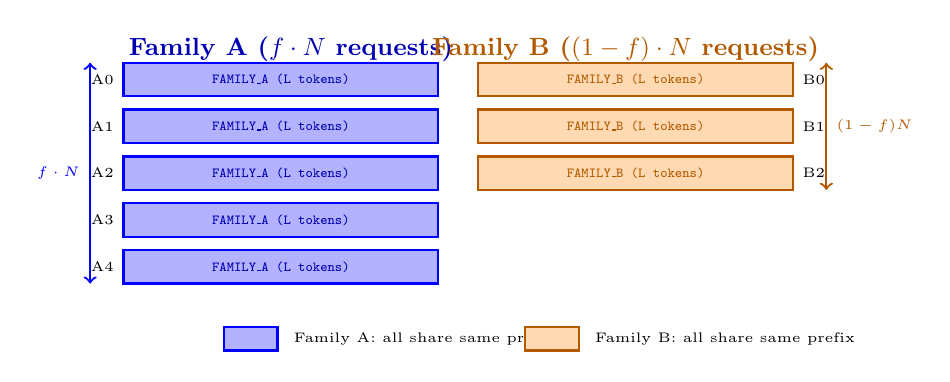
\begin{tikzpicture}[
    scale=0.85,
    every node/.style={font=\footnotesize}
]
% Parameters
\def\totalwidth{10}
\def\fraction{0.6}  % f = 0.6 (60% family A)
\pgfmathsetmacro{\halfwidth}{\totalwidth/2}
\pgfmathsetmacro{\leftwidth}{\halfwidth - 0.3}
\pgfmathsetmacro{\rightstart}{\halfwidth + 0.3}
\pgfmathsetmacro{\rightwidth}{\halfwidth - 0.3}
\def\boxheight{0.5}
\def\spacing{0.2}

% Title annotations
\node[font=\small\bfseries, blue!70!black] at (2.5, 2.5) {Family A ($f \cdot N$ requests)};
\node[font=\small\bfseries, orange!70!black] at (7.5, 2.5) {Family B ($(1-f) \cdot N$ requests)};

% Draw Family A requests
\foreach \i in {0,1,2,3,4} {
    \pgfmathsetmacro{\ypos}{1.8 - \i*(\boxheight + \spacing)}
    
    % Family A - all identical
    \fill[blue!30] (0, \ypos) rectangle (\leftwidth, \ypos + \boxheight);
    \draw[thick, blue] (0, \ypos) rectangle (\leftwidth, \ypos + \boxheight);
    
    % Label
    \node[left, font=\tiny] at (0, \ypos + \boxheight/2) {A\i};
    
    % Text inside
    \pgfmathsetmacro{\centerA}{\leftwidth/2}
    \node[blue!70!black, font=\tiny] at (\centerA, \ypos + \boxheight/2) {\texttt{FAMILY\_A (L tokens)}};
}

% Draw Family B requests
\foreach \i in {0,1,2} {
    \pgfmathsetmacro{\ypos}{1.8 - \i*(\boxheight + \spacing)}
    
    % Family B - all identical (but different from A)
    \fill[orange!30] (\rightstart, \ypos) rectangle (\totalwidth, \ypos + \boxheight);
    \draw[thick, orange!70!black] (\rightstart, \ypos) rectangle (\totalwidth, \ypos + \boxheight);
    
    % Label
    \node[right, font=\tiny] at (\totalwidth, \ypos + \boxheight/2) {B\i};
    
    % Text inside
    \pgfmathsetmacro{\centerB}{\rightstart + \rightwidth/2}
    \node[orange!70!black, font=\tiny] at (\centerB, \ypos + \boxheight/2) {\texttt{FAMILY\_B (L tokens)}};
}

% Annotations for counts
\pgfmathsetmacro{\topA}{1.8 + \boxheight}
\pgfmathsetmacro{\bottomA}{1.8 - 4*(\boxheight + \spacing)}
\draw[<->, thick, blue] (-0.5, \topA) -- (-0.5, \bottomA) 
    node[midway, left, font=\tiny] {$f \cdot N$};

\pgfmathsetmacro{\bottomB}{1.8 - 2*(\boxheight + \spacing)}    
\draw[<->, thick, orange!70!black] (\totalwidth + 0.5, \topA) -- (\totalwidth + 0.5, \bottomB) 
    node[midway, right, font=\tiny] {$(1-f) N$};

\fill[blue!30] (1.5, -2) rectangle ++(0.8, 0.35);
\draw[thick, blue] (1.5, -2) rectangle ++(0.8, 0.35);
\node[right, font=\tiny] at (2.4, -1.825) {Family A: all share same prefix};

\fill[orange!30] (6, -2) rectangle ++(0.8, 0.35);
\draw[thick, orange!70!black] (6, -2) rectangle ++(0.8, 0.35);
\node[right, font=\tiny] at (6.9, -1.825) {Family B: all share same prefix};

\end{tikzpicture}

\vspace{0.2cm}


{Two Family Batch Mixture (L = 100 tokens)}
    \begin{figure}
        \centering
    \includegraphics[width=\columnwidth]{\RESULTDIR/two_family_fraction_A_100.png}
    \captionof{figure}{Results across fraction of requests from A}
\end{figure}


{Two Family Batch Mixture (L = 500 tokens)}
    \begin{figure}
        \centering
    \includegraphics[width=\columnwidth]{\RESULTDIR/two_family_fraction_A_500.png}
    \captionof{figure}{Results across fraction of requests from A}
\end{figure}


{Two Family Batch Mixture (L = 1000 tokens)}
    \begin{figure}
        \centering
    \includegraphics[width=\columnwidth]{\RESULTDIR/two_family_fraction_A_1000.png}
    \captionof{figure}{Results across fraction of requests from A}
\end{figure}


{Two Family Batch Mixture (L = 2000 tokens)}
    \begin{figure}
        \centering
    \includegraphics[width=\columnwidth]{\RESULTDIR/two_family_fraction_A_2000.png}
    \captionof{figure}{Results across fraction of requests from A}
\end{figure}


{Tiered prefix sharing}
\centering
\begin{tikzpicture}[
    scale=0.85,
    every node/.style={font=\footnotesize}
]
% Parameters
\def\totalwidth{10}
\def\commonfrac{0.67}  % 2/3 of L is common
\pgfmathsetmacro{\commonwidth}{\totalwidth * \commonfrac}
\pgfmathsetmacro{\suffixwidth}{\totalwidth * (1-\commonfrac)}
\def\boxheight{0.5}
\def\spacing{0.2}
\def\fraction{0.6} 

\draw[<->, thick] (0, 2.7) -- (\totalwidth, 2.7) node[midway, above] {Total Length $L$ tokens};

\draw[<->, thick, blue] (0, 1.8) -- (\commonwidth, 1.8) node[midway, above, blue] {$\frac{2L}{3}$ common};


\draw[<->, thick, red] (\commonwidth, 1.8) -- (\totalwidth, 1.8) node[midway, above, red] {$\frac{L}{3}$ suffix};

\foreach \i in {0,1,2} {
    \pgfmathsetmacro{\ypos}{0.9 - \i*(\boxheight + \spacing)}
    
    \fill[blue!30] (0, \ypos) rectangle (\commonwidth, \ypos + \boxheight);
    \draw[thick, blue] (0, \ypos) rectangle (\commonwidth, \ypos + \boxheight);
    
    \fill[green!30] (\commonwidth, \ypos) rectangle (\totalwidth, \ypos + \boxheight);
    \draw[thick, green!60!black] (\commonwidth, \ypos) rectangle (\totalwidth, \ypos + \boxheight);
    
    \node[left, font=\tiny] at (-0.2, \ypos + \boxheight/2) {Req \i};
    
    \pgfmathsetmacro{\centerCommon}{\commonwidth/2}
    \pgfmathsetmacro{\centerSuffix}{\commonwidth + \suffixwidth/2}
    \node[blue!70!black, font=\tiny] at (\centerCommon, \ypos + \boxheight/2) {\texttt{COMMON}};
    \node[green!60!black, font=\tiny] at (\centerSuffix, \ypos + \boxheight/2) {\texttt{F\_SHARED}};
}

\foreach \i in {3,4} {
    \pgfmathsetmacro{\ypos}{0.9 - \i*(\boxheight + \spacing)}
    
    \fill[blue!30] (0, \ypos) rectangle (\commonwidth, \ypos + \boxheight);
    \draw[thick, blue] (0, \ypos) rectangle (\commonwidth, \ypos + \boxheight);
    
    \pgfmathsetmacro{\patternIdx}{int(\i-3)}
    \ifnum\patternIdx=0
        \fill[orange!20, pattern=north east lines, pattern color=orange!60] (\commonwidth, \ypos) rectangle (\totalwidth, \ypos + \boxheight);
    \fi
    \ifnum\patternIdx=1
        \fill[orange!20, pattern=north west lines, pattern color=orange!60] (\commonwidth, \ypos) rectangle (\totalwidth, \ypos + \boxheight);
    \fi
    \draw[thick, orange!70!black] (\commonwidth, \ypos) rectangle (\totalwidth, \ypos + \boxheight);
    
    \node[left, font=\tiny] at (-0.2, \ypos + \boxheight/2) {Req \i};
    
    \pgfmathsetmacro{\centerCommon}{\commonwidth/2}
    \pgfmathsetmacro{\centerSuffix}{\commonwidth + \suffixwidth/2}
    \node[blue!70!black, font=\tiny] at (\centerCommon, \ypos + \boxheight/2) {\texttt{COMMON}};
    \node[orange!70!black, font=\tiny] at (\centerSuffix, \ypos + \boxheight/2) {\texttt{U\i}};
}

\pgfmathsetmacro{\topShared}{0.9 + \boxheight}
\pgfmathsetmacro{\bottomShared}{0.9 - 2*(\boxheight + \spacing)}
\draw[<->, thick, green!60!black] (\totalwidth + 0.3, \topShared) -- (\totalwidth + 0.3, \bottomShared) 
    node[midway, right, font=\tiny] {$f \cdot N$};

\pgfmathsetmacro{\topUnique}{0.9 - 3*(\boxheight + \spacing) + \boxheight}
\pgfmathsetmacro{\bottomUnique}{0.9 - 4*(\boxheight + \spacing)}
\draw[<->, thick, orange!70!black] (\totalwidth + 0.3, \topUnique) -- (\totalwidth + 0.3, \bottomUnique) 
    node[midway, right, font=\tiny] {$(1-f) N$};


\fill[blue!30] (0.5, -3.3) rectangle ++(0.7, 0.35);
\draw[thick, blue] (0.5, -3.3) rectangle ++(0.7, 0.35);
\node[right, font=\tiny] at (1.3, -3.125) {Common prefix (all)};

\fill[green!30] (3.8, -3.3) rectangle ++(0.7, 0.35);
\draw[thick, green!60!black] (3.8, -3.3) rectangle ++(0.7, 0.35);
\node[right, font=\tiny] at (4.6, -3.125) {Shared suffix ($f \cdot N$)};

\fill[orange!20, pattern=north east lines, pattern color=orange!60] (7.3, -3.3) rectangle ++(0.7, 0.35);
\draw[thick, orange!70!black] (7.3, -3.3) rectangle ++(0.7, 0.35);
\node[right, font=\tiny] at (8.1, -3.125) {Unique suffixes};

\end{tikzpicture}

\vspace{0.2cm}


{Tiered Prefix Sharing (L = 500 tokens)}
    \begin{figure}
        \centering
    \includegraphics[width=\columnwidth]{\RESULTDIR/fraction_on_lower_tier_500.png}
    \captionof{figure}{Varying fraction on lowermost tier}
\end{figure}


{Tiered Prefix Sharing (L = 2000 tokens)}
    \begin{figure}
        \centering
    \includegraphics[width=\columnwidth]{\RESULTDIR/fraction_on_lower_tier_2000.png}
    \captionof{figure}{Varying fraction on lowermost tier}
\end{figure}



{Throughput vs Max Batch Size}
    \begin{figure}
        \centering
    \includegraphics[width=\columnwidth]{\RESULTDIR/throughput_vs_max_batch_size_1200.png}
    \captionof{figure}{Throughput vs Max Batch Size (L = 1200 tokens)}
\end{figure}


{Two Family Mixture - Mean DRAM Activity}
    \begin{figure}
        \centering
    \includegraphics[width=\columnwidth]{\RESULTDIR/mean_dram_act_frac_a_2000.png}
    \captionof{figure}{Mean DRAM Activity across fraction of requests from A (L = 2000 tokens)}
\end{figure}


{Two Family Mixture - Total DRAM Accesses}
    \begin{figure}
        \centering
    \includegraphics[width=\columnwidth]{\RESULTDIR/total_dram_acccesses_frac_a_2000.png}
    \captionof{figure}{Total DRAM Accesses across fraction of requests from A (L = 2000 tokens)}
\end{figure}



{Two Family Mixture - Mean SM Activity}
    \begin{figure}
        \centering
    \includegraphics[width=\columnwidth]{\RESULTDIR/sm_act_frac_a_2000.png}
    \captionof{figure}{Mean SM Activity across fraction of requests from A (L = 2000 tokens)}
\end{figure}


{Two Family Mixture - Mean SM Occupancy}
    \begin{figure}
        \centering
    \includegraphics[width=\columnwidth]{\RESULTDIR/sm_occ_frac_a_2000.png}
    \captionof{figure}{Mean SM Occupancy across fraction of requests from A (L = 2000 tokens)}
\end{figure}


{Two Family Mixture - Mean Tensor Core Utilization}
    \begin{figure}
        \centering
    \includegraphics[width=\columnwidth]{\RESULTDIR/tenso_frac_a_2000.png}
    \captionof{figure}{Mean Tensor Core Utilization across fraction of requests from A (L = 2000 tokens)}
\end{figure}




{Tiered Prefix Sharing}
\centering
\begin{tikzpicture}[
    scale=0.85,
    every node/.style={font=\footnotesize}
]
% Parameters
\def\totalwidth{10}
\def\commonfrac{0.667}   % f1: fraction of L that is common prefix
\def\f{0.5}              % f2: fraction of N assigned to family 1
\def\numfamilies{6}      % total families (1 dominant + 5 others)
\pgfmathsetmacro{\commonwidth}{\totalwidth * \commonfrac}
\pgfmathsetmacro{\suffixwidth}{\totalwidth * (1-\commonfrac)}
\def\boxheight{0.5}
\def\spacing{0.2}

% ── top rulers ──────────────────────────────────────────────────────────────
\draw[<->, thick]
    (0, 2.8) -- (\totalwidth, 2.8)
    node[midway, above] {Total prompt length $L$ tokens};

\draw[<->, thick, blue]
    (0, 1.9) -- (\commonwidth, 1.9)
    node[midway, above, blue] {$f_1 L$ \ common prefix};

\draw[<->, thick, red]
    (\commonwidth, 1.9) -- (\totalwidth, 1.9)
    node[midway, above, red] {$(1{-}f_1)L$ \ family suffix};

% ── Family 1 rows (dominant family, f2*N requests) ───────────────────────
% We draw 3 representative rows
\foreach \i in {0,1,2} {
    \pgfmathsetmacro{\ypos}{0.9 - \i*(\boxheight + \spacing)}

    % Common prefix segment
    \fill[blue!30]  (0, \ypos) rectangle (\commonwidth, \ypos+\boxheight);
    \draw[thick, blue] (0, \ypos) rectangle (\commonwidth, \ypos+\boxheight);

    % Family-1 shared suffix
    \fill[green!30] (\commonwidth, \ypos) rectangle (\totalwidth, \ypos+\boxheight);
    \draw[thick, green!60!black] (\commonwidth, \ypos) rectangle (\totalwidth, \ypos+\boxheight);

    \node[left, font=\tiny] at (-0.2, \ypos+\boxheight/2) {Req \i};
    \pgfmathsetmacro{\cx}{\commonwidth/2}
    \pgfmathsetmacro{\sx}{\commonwidth + \suffixwidth/2}
    \node[blue!70!black,  font=\tiny] at (\cx, \ypos+\boxheight/2) {\texttt{COMMON}};
    \node[green!60!black, font=\tiny] at (\sx, \ypos+\boxheight/2) {\texttt{FAM1}};
}

% ── Other-family rows (5 families, each with unique suffix) ──────────────
% We draw 2 representative rows (one per other family shown)
\foreach \i in {3,4} {
    \pgfmathsetmacro{\ypos}{0.9 - \i*(\boxheight + \spacing)}
    \pgfmathsetmacro{\famnum}{int(\i-1)}   % FAM2, FAM3, ...

    % Common prefix segment
    \fill[blue!30]  (0, \ypos) rectangle (\commonwidth, \ypos+\boxheight);
    \draw[thick, blue] (0, \ypos) rectangle (\commonwidth, \ypos+\boxheight);

    % Unique suffix (hatched orange, different pattern per row)
    \pgfmathsetmacro{\patternIdx}{int(\i-3)}
    \ifnum\patternIdx=0
        \fill[orange!20, pattern=north east lines, pattern color=orange!60]
            (\commonwidth, \ypos) rectangle (\totalwidth, \ypos+\boxheight);
    \fi
    \ifnum\patternIdx=1
        \fill[orange!20, pattern=north west lines, pattern color=orange!60]
            (\commonwidth, \ypos) rectangle (\totalwidth, \ypos+\boxheight);
    \fi
    \draw[thick, orange!70!black] (\commonwidth, \ypos) rectangle (\totalwidth, \ypos+\boxheight);

    \node[left, font=\tiny] at (-0.2, \ypos+\boxheight/2) {Req \i};
    \pgfmathsetmacro{\cx}{\commonwidth/2}
    \pgfmathsetmacro{\sx}{\commonwidth + \suffixwidth/2}
    \node[blue!70!black,   font=\tiny] at (\cx, \ypos+\boxheight/2) {\texttt{COMMON}};
    \node[orange!70!black, font=\tiny] at (\sx, \ypos+\boxheight/2) {\texttt{FAM\famnum}};
}

% ── Right-side braces showing request counts ─────────────────────────────
% Family-1 brace  (rows 0..2)
\pgfmathsetmacro{\topF}{0.9 + \boxheight}
\pgfmathsetmacro{\botF}{0.9 - 2*(\boxheight + \spacing)}
\draw[<->, thick, green!60!black]
    (\totalwidth+0.3, \topF) -- (\totalwidth+0.3, \botF)
    node[midway, right, font=\tiny] {$f_2 N$};

% Other-families brace  (rows 3..4)
\pgfmathsetmacro{\topO}{0.9 - 3*(\boxheight+\spacing) + \boxheight}
\pgfmathsetmacro{\botO}{0.9 - 4*(\boxheight+\spacing)}
\draw[<->, thick, orange!70!black]
    (\totalwidth+0.3, \topO) -- (\totalwidth+0.3, \botO)
    node[midway, right, font=\tiny]
    {$\frac{(1{-}f_2)N}{K{-}1}$ each};

% ── Legend ───────────────────────────────────────────────────────────────
\fill[blue!30]   (0.3,-3.2) rectangle ++(0.7,0.35);
\draw[thick,blue](0.3,-3.2) rectangle ++(0.7,0.35);
\node[right, font=\tiny] at (1.1,-3.025)
    {Common prefix — shared by \emph{all} $N$ requests ($f_1 L$ tokens)};

\fill[green!30]  (0.3,-3.7) rectangle ++(0.7,0.35);
\draw[thick,green!60!black](0.3,-3.7) rectangle ++(0.7,0.35);
\node[right, font=\tiny] at (1.1,-3.525)
    {Family-1 suffix — shared by $f_2 N$ requests (dominant family)};

\fill[orange!20, pattern=north east lines, pattern color=orange!60]
    (0.3,-4.2) rectangle ++(0.7,0.35);
\draw[thick,orange!70!black](0.3,-4.2) rectangle ++(0.7,0.35);
\node[right, font=\tiny] at (1.1,-4.025)
    {Unique family suffix — $K{-}1$ minority families, $\frac{(1-f_2)N}{K-1}$ reqs each};

\end{tikzpicture}
\vspace{0.2cm}


{Tiered Prefix Sharing (L = 2000 tokens) (Number of families = 6)}
    \begin{figure}
        \centering
    \includegraphics[width=\columnwidth]{\RESULTDIR/tiered_prefix_sharing_2000_fam_6_f1_f2.png}
\end{figure}


{Tiered Prefix Sharing (L = 10000 tokens) (Number of families = 6)}
    \begin{figure}
        \centering
    \includegraphics[width=\columnwidth]{\RESULTDIR/tiered_prefix_sharing_10000_fam_6_f1_f2.png}
\end{figure}


{Tiered Prefix Sharing (L = 2000 tokens) (Number of families = 51)}
    \begin{figure}
        \centering
    \includegraphics[width=\columnwidth]{\RESULTDIR/tiered_prefix_sharing_2000_fam_51_f1_f2.png}
\end{figure}


{Tiered Prefix Sharing (L = 10000 tokens) (Number of families = 51)}
    \begin{figure}
        \centering
    \includegraphics[width=\columnwidth]{\RESULTDIR/tiered_prefix_sharing_10000_fam_51_f1_f2.png}
\end{figure}


{Varying the amount of sharing}
\centering
\begin{tikzpicture}[
    scale=0.85,
    every node/.style={font=\footnotesize}
]

\def\totalwidth{10}
\def\fraction{0.5} 
\pgfmathsetmacro{\sharedwidth}{\totalwidth * \fraction}
\pgfmathsetmacro{\uniquewidth}{\totalwidth * (1-\fraction)}
\def\boxheight{0.5}
\def\spacing{0.2}

\draw[<->, thick] (0, 2.2) -- (\totalwidth, 2.2) node[midway, above] {Total Length $L$ tokens};

\draw[<->, thick, blue] (0, 1.8) -- (\sharedwidth, 1.8) node[midway, above, blue] {$f \cdot L$};

\draw[<->, thick, red] (\sharedwidth, 1.8) -- (\totalwidth, 1.8) node[midway, above, red] {$(1-f) \cdot L$};

\foreach \i in {0,1,2,3,4} {
    \pgfmathsetmacro{\ypos}{1.2 - \i*(\boxheight + \spacing)}
    
    \fill[blue!30] (0, \ypos) rectangle (\sharedwidth, \ypos + \boxheight);
    \draw[thick, blue] (0, \ypos) rectangle (\sharedwidth, \ypos + \boxheight);
    
    \ifnum\i=0
        \fill[red!20, pattern=north east lines, pattern color=red!50] (\sharedwidth, \ypos) rectangle (\totalwidth, \ypos + \boxheight);
    \fi
    \ifnum\i=1
        \fill[red!20, pattern=north west lines, pattern color=red!50] (\sharedwidth, \ypos) rectangle (\totalwidth, \ypos + \boxheight);
    \fi
    \ifnum\i=2
        \fill[red!20, pattern=horizontal lines, pattern color=red!50] (\sharedwidth, \ypos) rectangle (\totalwidth, \ypos + \boxheight);
    \fi
    \ifnum\i=3
        \fill[red!20, pattern=vertical lines, pattern color=red!50] (\sharedwidth, \ypos) rectangle (\totalwidth, \ypos + \boxheight);
    \fi
    \ifnum\i=4
        \fill[red!20, pattern=dots, pattern color=red!50] (\sharedwidth, \ypos) rectangle (\totalwidth, \ypos + \boxheight);
    \fi
    \draw[thick, red] (\sharedwidth, \ypos) rectangle (\totalwidth, \ypos + \boxheight);
    
    \node[left, font=\tiny] at (-0.2, \ypos + \boxheight/2) {Req \i};
    
    \node[blue!70!black, font=\tiny] at (\sharedwidth/2, \ypos + \boxheight/2) {\texttt{SHARED}};
    \node[red!70!black, font=\tiny] at (\sharedwidth + \uniquewidth/2, \ypos + \boxheight/2) {\texttt{U\i}};
}


\fill[blue!30] (1, -2.8) rectangle ++(0.8, 0.35);
\draw[thick, blue] (1, -2.8) rectangle ++(0.8, 0.35);
\node[right, font=\tiny] at (1.9, -2.625) {Shared prefix};

\fill[red!20, pattern=north east lines, pattern color=red!50] (6.5, -2.8) rectangle ++(0.8, 0.35);
\draw[thick, red] (6.5, -2.8) rectangle ++(0.8, 0.35);
\node[right, font=\tiny] at (7.4, -2.625) {Unique per request};

\end{tikzpicture}

\vspace{0.3cm}



{Varying the amount of sharing - different RL Techniques}
    \begin{figure}
        \centering
    \includegraphics[width=\columnwidth]{\RESULTDIR/fraction_sharing_throughput_average_batch_size.png}
    \captionof{figure}{Throughput and Average Batch Sizes across Fractions ($L = 1200$ tokens, batch of $100$ requests)}
\end{figure}


{Varying the amount of sharing - different RL Techniques - average batch size (fraction = 0)}
    \begin{figure}
        \centering
    \includegraphics[width=\columnwidth]{\RESULTDIR/fraction_sharing_policies_0.png}
\end{figure}


{Varying the amount of sharing - different RL Techniques - average batch size (fraction = 0.2)}
    \begin{figure}
        \centering
    \includegraphics[width=\columnwidth]{\RESULTDIR/fraction_sharing_policies_0.2.png}
\end{figure}



{Varying the amount of sharing - different RL Techniques - average batch size (fraction = 0.4)}
    \begin{figure}
        \centering
    \includegraphics[width=\columnwidth]{\RESULTDIR/fraction_sharing_policies_0.4.png}
\end{figure}



{Varying the amount of sharing - different RL Techniques - average batch size (fraction = 0.6)}
    \begin{figure}
        \centering
    \includegraphics[width=\columnwidth]{\RESULTDIR/fraction_sharing_policies_0.6.png}
\end{figure}



{Varying the amount of sharing - different RL Techniques - average batch size (fraction = 0.8)}
    \begin{figure}
        \centering
    \includegraphics[width=\columnwidth]{\RESULTDIR/fraction_sharing_policies_0.8.png}
\end{figure}



{Varying the amount of sharing - different RL Techniques - average batch size (fraction = 1.0)}
    \begin{figure}
        \centering
    \includegraphics[width=\columnwidth]{\RESULTDIR/fraction_sharing_policies_1.0.png}
\end{figure}